\documentclass{vgtc}                          % final (conference style)
%\documentclass[review]{vgtc}                 % review
%\documentclass[widereview]{vgtc}             % wide-spaced review
%\documentclass[preprint]{vgtc}               % preprint
%\documentclass[electronic]{vgtc}             % electronic version

%% Uncomment one of the lines above depending on where your paper is
%% in the conference process. ``review'' and ``widereview'' are for review
%% submission, ``preprint'' is for pre-publication, and the final version
%% doesn't use a specific qualifier. Further, ``electronic'' includes
%% hyperreferences for more convenient online viewing.

%% Please use one of the ``review'' options in combination with the
%% assigned online id (see below) ONLY if your paper uses a double blind
%% review process. Some conferences, like IEEE Vis and InfoVis, have NOT
%% in the past.

%% Figures should be in CMYK or Grey scale format, otherwise, colour 
%% shifting may occur during the printing process.

%% These few lines make a distinction between latex and pdflatex calls and they
%% bring in essential packages for graphics and font handling.
%% Note that due to the \DeclareGraphicsExtensions{} call it is no longer necessary
%% to provide the the path and extension of a graphics file:
%% \includegraphics{diamondrule} is completely sufficient.
%%
\ifpdf%                                % if we use pdflatex
  \pdfoutput=1\relax                   % create PDFs from pdfLaTeX
  \pdfcompresslevel=9                  % PDF Compression
  \pdfoptionpdfminorversion=7          % create PDF 1.7
  \ExecuteOptions{pdftex}
  \usepackage{graphicx}                % allow us to embed graphics files
  \DeclareGraphicsExtensions{.pdf,.png,.jpg,.jpeg} % for pdflatex we expect .pdf, .png, or .jpg files
\else%                                 % else we use pure latex
  \ExecuteOptions{dvips}
  \usepackage{graphicx}                % allow us to embed graphics files
  \DeclareGraphicsExtensions{.eps}     % for pure latex we expect eps files
\fi%

%% it is recomended to use ``\autoref{sec:bla}'' instead of ``Fig.~\ref{sec:bla}''
\graphicspath{{figures/}{pictures/}{images/}{./}} % where to search for the images

\usepackage{microtype}                 % use micro-typography (slightly more compact, better to read)
\PassOptionsToPackage{warn}{textcomp}  % to address font issues with \textrightarrow
\usepackage{textcomp}                  % use better special symbols
\usepackage{mathptmx}                  % use matching math font
\usepackage{times}                     % we use Times as the main font
\renewcommand*\ttdefault{txtt}         % a nicer typewriter font
\usepackage{cite}                      % needed to automatically sort the references
\usepackage{tabu}                      % only used for the table example
\usepackage{booktabs}                  % only used for the table example
\usepackage{amsmath}                   % align
\usepackage{algorithm}                 % use for algorithms
\usepackage[noend]{algpseudocode}      % use for algorithms
\usepackage{dblfloatfix}               % figures at bottom of page
\usepackage{makecell}                  % for cells in a table
\usepackage{arydshln}                  % for dashed separators in a table
\usepackage{textcomp}                  % proper tilde (~)
\newcommand{\textapprox}{\raisebox{0.5ex}{\texttildelow}}
\usepackage{color}
\definecolor{small_scale}{RGB}{16, 61, 135}
\definecolor{large_scale}{RGB}{153, 6, 6}
%% We encourage the use of mathptmx for consistent usage of times font
%% throughout the proceedings. However, if you encounter conflicts
%% with other math-related packages, you may want to disable it.

% declaration of the new block
\algblock{ParFor}{EndParFor}
% customising the new block
\algnewcommand\algorithmicparfor{\textbf{parfor}}
\algnewcommand\algorithmicpardo{\textbf{do}}
\algnewcommand\algorithmicendparfor{\textbf{end\ parfor}}
\algrenewtext{ParFor}[1]{\algorithmicparfor\ #1\ \algorithmicpardo}
\algrenewtext{EndParFor}{\algorithmicendparfor}

% continuation indent patch http://tex.stackexchange.com/questions/78776/forced-indentation-in-algorithmicx
\newlength{\continueindent}
\setlength{\continueindent}{2em}
\usepackage{etoolbox}
\makeatletter
\newcommand*{\ALG@customparshape}{\parshape 2 \leftmargin \linewidth \dimexpr\ALG@tlm+\continueindent\relax \dimexpr\linewidth+\leftmargin-\ALG@tlm-\continueindent\relax}
\apptocmd{\ALG@beginblock}{\ALG@customparshape}{}{\errmessage{failed to patch}}
\makeatother
% end continuation indent patch

\makeatletter
\newcommand\fs@betterruled{%
  \def\@fs@cfont{\bfseries}\let\@fs@capt\floatc@ruled
  \def\@fs@pre{\vspace*{5pt}\hrule height.8pt depth0pt \kern2pt}%
  \def\@fs@post{\kern2pt\hrule\relax}%
  \def\@fs@mid{\kern2pt\hrule\kern2pt}%
  \let\@fs@iftopcapt\iftrue}
\floatstyle{betterruled}
\restylefloat{algorithm}
\makeatother

\newcommand{\setalglineno}[1]{%
  \setcounter{ALG@line}{\numexpr#1-1}}

\newcommand{\algorithmautorefname}{Algorithm}

%% If you are submitting a paper to a conference for review with a double
%% blind reviewing process, please replace the value ``0'' below with your
%% OnlineID. Otherwise, you may safely leave it at ``0''.
\onlineid{0}

%% declare the category of your paper, only shown in review mode
\vgtccategory{Research}

%% allow for this line if you want the electronic option to work properly
\vgtcinsertpkg

%% In preprint mode you may define your own headline. If not, the default IEEE copyright message will appear in preprint mode.
%\preprinttext{To appear in an IEEE VGTC sponsored conference.}

%% This adds a link to the version of the paper on IEEEXplore
%% Uncomment this line when you produce a preprint version of the article 
%% after the article receives a DOI for the paper from IEEE
%\ieeedoi{xx.xxxx/TVCG.201x.xxxxxxx}


%% Paper title.
\title{GPU-based Image Compression for Efficient Compositing\texorpdfstring{\\}{ }in Distributed Rendering Applications }

%% This is how authors are specified in the conference style

%% Author and Affiliation (single author).
%%\author{Roy G. Biv\thanks{e-mail: roy.g.biv@aol.com}}
%%\affiliation{\scriptsize Allied Widgets Research}

%% Author and Affiliation (multiple authors with single affiliations).
%%\author{Roy G. Biv\thanks{e-mail: roy.g.biv@aol.com} %
%%\and Ed Grimley\thanks{e-mail:ed.grimley@aol.com} %
%%\and Martha Stewart\thanks{e-mail:martha.stewart@marthastewart.com}}
%%\affiliation{\scriptsize Martha Stewart Enterprises \\ Microsoft Research}

%% Author and Affiliation (multiple authors with multiple affiliations)
\author{Riley Lipinksi\thanks{e-mail: lipi8497@stthomas.edu}\\ %
     \scriptsize University of St. Thomas %
\and Kenneth Moreland\thanks{e-mail: morelandkd@ornl.gov}\\ %
     \scriptsize Oak Ridge National Laboratory %
\and Michael E. Papka\thanks{e-mail: papka@anl.gov}\\ %
     \parbox{1.4in}{\scriptsize \centering Argonne National Laboratory \\ Northern Illinois University}
\and Thomas Marrinan\thanks{e-mail: tmarrinan@stthomas.edu}\\ %
     \parbox{1.4in}{\scriptsize \centering University of St. Thomas \\ Argonne National Laboratory}}
     
%% Abstract section.
\abstract{Visualizations of large-scale data sets are often created on graphics clusters that distribute the rendering task amongst many processes. When using real-time GPU-based graphics algorithms, the most time-consuming aspect of distributed rendering is typically the compositing phase -- combining all partial images from each rendering process into the final visualization. Compositing requires image data to be copied off the GPU and sent over a network to other processes. While compression has been utilized in existing distributed rendering compositors to reduce the data being sent over the network, this compression tends to occur after the raw images are transferred from the GPU to main memory. In this paper, we present work that leverages OpenGL / CUDA interoperability to compress raw images on the GPU prior to transferring the data to main memory. This approach can significantly reduce the device-to-host data transfer time, thus enabling more efficient compositing of images generated by distributed rendering applications.}

%% ACM Computing Classification System (CCS). 
%% See <http://www.acm.org/about/class> for details.
%% We recommend the 2012 system <http://www.acm.org/about/class/class/2012>
%% For the 2012 system use the ``\CCScatTwelve'' which command takes four arguments.
%% The 1998 system <http://www.acm.org/about/class/class/2012> is still possible
%% For the 1998 system use the ``\CCScat'' which command takes four arguments.
%% In both cases the last two arguments (1998) or last three (2012) can be empty.

\CCScatlist{
  \CCScatTwelve{Computing methodologies}{Computer graphics}{Image compression}{};
  \CCScatTwelve{Computing methodologies}{Parallel computing methodologies}{Parallel algorithms}{Massively parallel algorithms}
}

%\CCScatlist{
  %\CCScat{H.5.2}{User Interfaces}{User Interfaces}{Graphical user interfaces (GUI)}{};
  %\CCScat{H.5.m}{Information Interfaces and Presentation}{Miscellaneous}{}{}
%}

%% Copyright space is enabled by default as required by guidelines.
%% It is disabled by the 'review' option or via the following command:
% \nocopyrightspace

%%%%%%%%%%%%%%%%%%%%%%%%%%%%%%%%%%%%%%%%%%%%%%%%%%%%%%%%%%%%%%%%
%%%%%%%%%%%%%%%%%%%%%% START OF THE PAPER %%%%%%%%%%%%%%%%%%%%%%
%%%%%%%%%%%%%%%%%%%%%%%%%%%%%%%%%%%%%%%%%%%%%%%%%%%%%%%%%%%%%%%%
\begin{document}

\setlength{\abovedisplayskip}{0pt} % fix spacing above equations
\setlength{\belowdisplayskip}{12pt} % fix spacing above equations

%% The ``\maketitle'' command must be the first command after the
%% ``\begin{document}'' command. It prepares and prints the title block.

%% the only exception to this rule is the \firstsection command
\firstsection{Introduction}

\maketitle

Data sets produced by simulations and collected from digital instruments and sensors are often too large to analyze on a single computer. Instead, researchers tend to leverage remote High-Performance Computing (HPC) centers where work can be distributed amongst many nodes of a computational resource. One common analysis task that researchers leverage to gain an understanding of the underlying data is three-dimensional (3D) visualization \cite{Stahli_2018, Taylor_2000}. 

Creating large-scale visualizations depends on distributed rendering applications that are capable of splitting geometric data between multiple GPUs (usually on multiple nodes of a graphics cluster).
Multiple approaches to distributing rendering on parallel nodes exist \cite{Molnar1994}, but the most fitting for large-scale HPC use an image compositing technique \cite{Wylie2001}.
In this approach, partial images are rendered independently on each process in the distributed rendering task. The partial images are then composited into the final visualization (example shown in \autoref{fig:intro}). When using real-time graphics algorithms, this compositing phase is typically the bottleneck in distributed rendering applications for two reasons: 1) rendered partial images must be copied from GPU memory to main memory, and 2) images now in main memory of each rendering process must be sent between rendering processes via network interconnect. This overhead can significantly increase overall job time and inhibit the ability to achieve interactive frame rates when streaming for real-time viewing and interaction \cite{Eilemann_2020, Moreland_2011}.

\begin{figure}[tb]
 \centering
 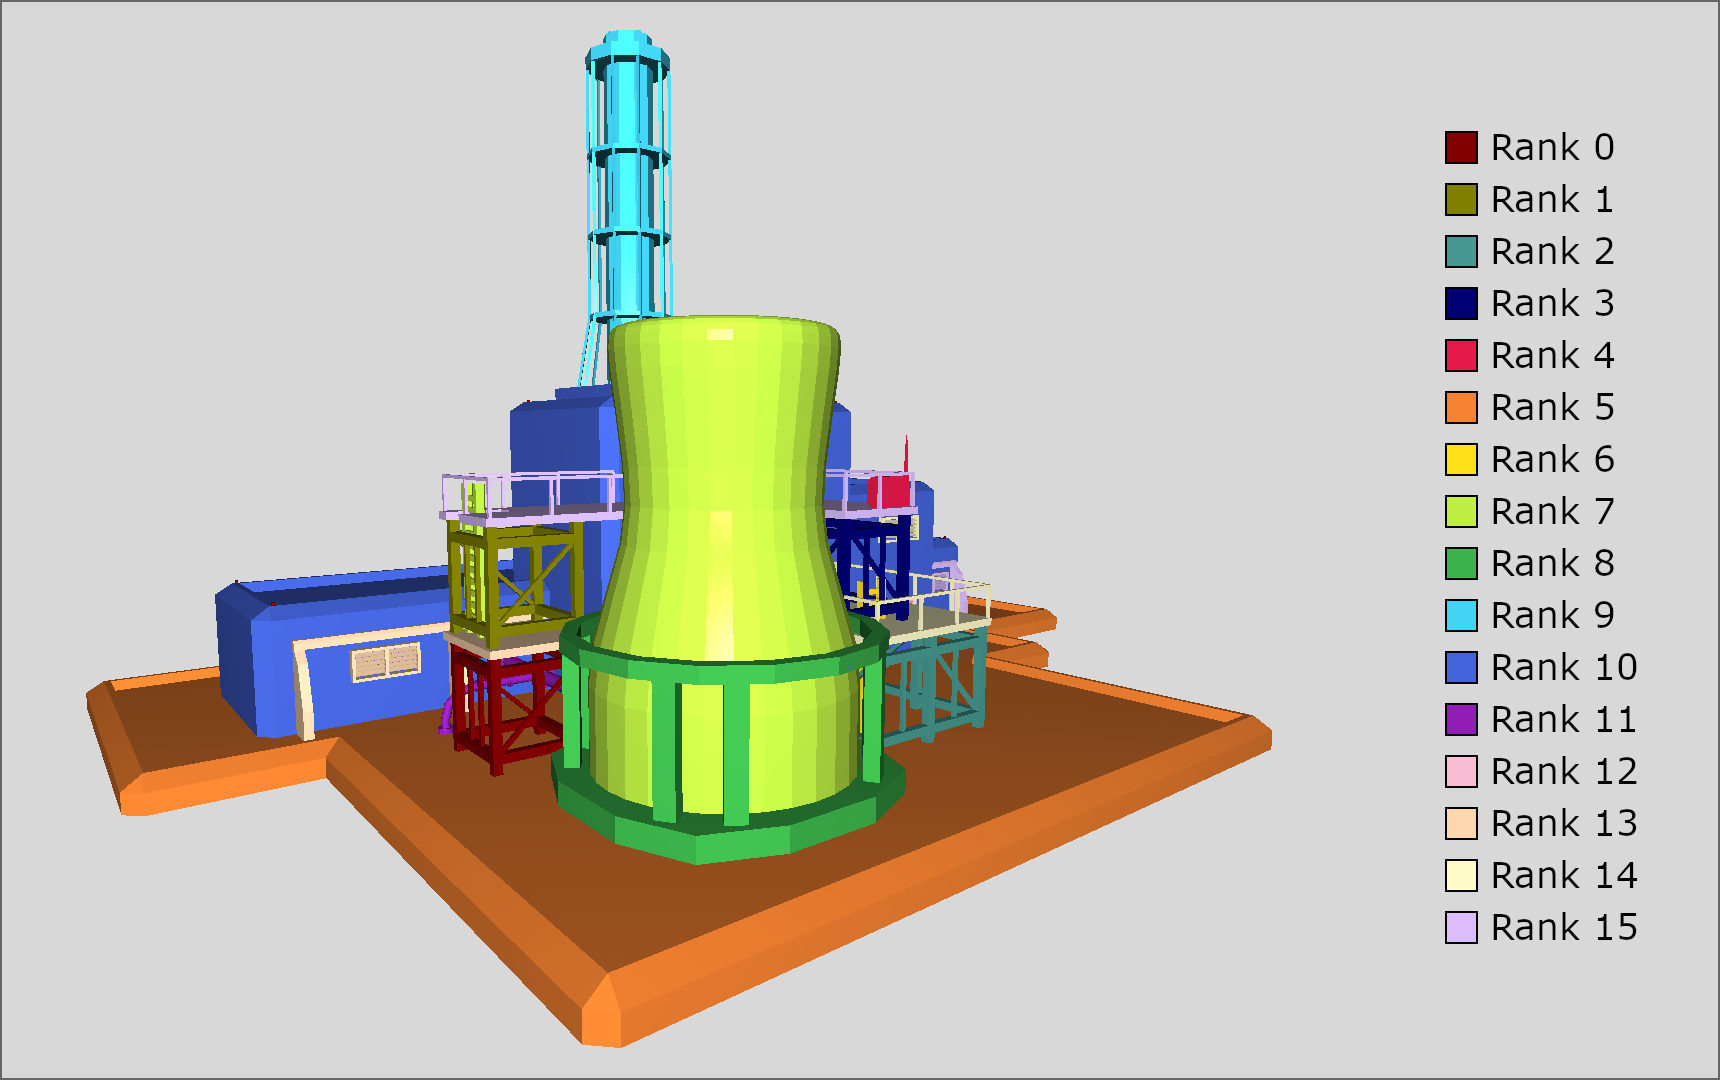
\includegraphics[width=\columnwidth]{figures/IceT_NuclearStation_ColorByRank16.png}
 \caption{Composited rendering of a nuclear power station using 16 processes. Each process has drawn its portion of the model using a unique color.}
 \label{fig:intro}
\end{figure}

While a few different distributed image compositors exist, IceT \cite{IceT_UserGuide, Moreland_2011} serves as an industry standard and has been integrated into widely used distributed rendering applications such as ParaView \cite{ParaView} and VisIt \cite{VisIt}. Prior to our work, IceT did leverage a form of compression for sending image data between rendering processes, but it still required copying uncompressed color and depth data from each rendering process's GPU to main memory. Our work aimed to implement image compression on the GPU, which yielded two benefits: 1) faster compression by leveraging the parallel architecture of GPUs, and 2) smaller data transfer size between a GPU and its host's main memory.

After covering prior related work on distributed rendering and compositing, this paper describes the GPU implementation of IceT's \textit{Active Pixel} image compression format -- a form of run-length encoding that accounts for image depth in addition to color. Next, it covers updates made to the IceT library to support modern OpenGL applications and GPU-based image compression. After describing implementation details, a series of performance measurements are provided in order to demonstrate the impact of GPU-based image compression on compositing in distributed rendering applications. Finally, the paper will conclude with limitations and of this work and future improvements to be made.


\section{Related Work}
As we aimed to integrate GPU-based image compression into a distributed rendering compositor, we investigated prior work done on distributed rendering and on image compression using GPUs.

\subsection{Distributed Rendering and Compositing}
Compositing images in distributed rendering applications occurs in one of two ways -- two-dimensional (2D) image space compositing (i.e. stitching sub-images together) or three-dimensional (3D) image space compositing (i.e. blending overlapping pixels).
In the former method, the output image is partitioned into 2D regions. Geometry is sent to the processor responsible for that region of image space and rendered locally. These regions are then stitched together for the final image.
In the latter method, the geometry is partitioned among processors, and each processors renders a full image with its portion of the geometry. These full images of partial geometry are blended together using a per-pixel operation that either blends colors or uses depth information to find the ``front'' color.

The image stitching approach is a natural fit for tiled displays, which partition the screen space with hardware \cite{Hereld2000}. Several rendering systems such as WireGL \cite{Humphreys_2001}, CGLX \cite{Doerr_2011}, and ClusterGL \cite{Neal2011} take advantage of this fact by intercepting OpenGL calls and streaming them to the appropriate nodes. Although these systems scale well with the size of the display, they suffer from potential load balancing problems with respect to the geometry.For example, if a model is only visible on two tiles, then only the two nodes responsible for rendering those tiles would receive the draw commands for that model.

To improve the load balancing of screen partitions, Samanta et al. \cite{Samanta1999} dynamically repartition the screen space.
Areas of the screen with more geometry are partitioned into smaller regions so that each region takes roughly the same amount of time to render.
These screen partitions then need to be read back, redistributed, and re-stitched to the physical display.
The idea is periodically rediscovered by other rendering systems \cite{Revanth_2012,Dong2019}.
Although this stitching approach only needs to handle color data, there is one major drawback -- geometric models can cross sub-image boundaries and therefore need to be loaded on multiple rendering nodes.

In contrast, the image compositing approach where a stack of images, each generated by a different process, are blended together pixel-by-pixel has a high initial overhead -- including reading back render buffers, transferring pixel data, and blending pixels -- but scales very well with respect to the size of data.
The approach is shown to work well at the largest scales \cite{Childs2010,Moreland_2011}.
Much of the work on image compositing focuses on the reduction network for the images \cite{Lin2004,Ma1994,Moreland2018,Nonaka2018,Peterka2009,Yu2008}, but there have been multiple other optimizations including amortizing costs across multiple renderings \cite{Larsen2016}, interlacing images for better load balancing \cite{Takeuchi2003}, improved gathering \cite{Grosset2017}, and of course compression \cite{Ahrens1998,Moreland_2001,Yang1999}, which is the focus of this paper.

Some rendering systems are designed for multiple modes of parallel rendering.
Chromium \cite{Humphreys_2002} extends the functionality of WireGL \cite{Humphreys_2001} to customize the streaming behavior of OpenGL calls, insert new behavior in the rendering system, and provide ``out of band'' communication to blend image pixels.
More recently, Equalizer \cite{Eilemann_2009,Eilemann_2020} serves as a full fledged distributed rendering framework that incorporates dynamic load balancing of geometry and supports advanced rendering techniques such as stereoscopy for CAVE virtual reality displays. For the image compositing portion of the distributed rendering task, Equalizer leverages region of interest detection and basic image compression to reduce the data sent between rendering processes. This enables distributed rendering applications based on Equalizer to achieve interactive frame rates.

IceT \cite{Moreland_2011} is an image compositing library that differentiates itself from other systems in a couple ways. First, when compared to other pixel blending systems, it reduces the time spent compositing by leveraging the fact that rendered sub-images often have significant empty space. This allows IceT to remove pixels in empty regions from inter-process communication, thus making better use of available network bandwidth. It also allows IceT to ignore the empty regions when compositing sub-images together, which reduces the computation time. Second, unlike Equalizer, it decouples itself from the rendering. This makes it more flexible so that it can work with a variety of rendering interfaces (including, but not limited to OpenGL).

\subsection{GPU-based Image Compression}
The primary purpose of most image compression algorithms is to reduce the image's data size while maintaining image quality. There are two types of image compression -- lossless and lossy. Lossless compressed images can be fully recovered to their original uncompressed state, whereas lossy compressed images cannot. In either case, compression speed is often left as a secondary goal at best. Thus many compression algorithms are not well suited for real-time distributed rendering and compositing.

One form of lossless image compression that is computationally efficient is run-length encoding (RLE) \cite{Robinson_1967}. RLE images group sequences of adjacent pixels with the same color by simply specifying the number of pixels in a run and the color for that run. RLE compression works particularly well when there are large swaths of uniform color in an image. Rutter \cite{Rutter_2011} created a parallel implementation of RLE compression that could be computed on a GPU. Although the computational complexity is increased from the serial version, the overall computation time is significantly reduced due to the massive parallelism provided by GPUs.

%Another lossless compression scheme is Lempel–Ziv–Welch (LZW) compression \cite{Welch_1984}. LZW compression works with any generic data type and has been implemented in common image formats such as TIFF and GIF. Generic data can be compressed using the LZW algorithm by treating a sequence of bytes as characters in a string. A dictionary is introduced that stores patterns / substrings found in the data. Any time a new pattern is found, it must be added to the dictionary. The final compressed data contains both the dictionary and the sequence of dictionary keys that matches the input data. LZW compression works particularly well when there are patterns that repeat frequently (whether sequentially or not). Funasaka et al. \cite{Funasaka_2015} has demonstrated that the LZW algorithm can be parallelized and executed on a GPU. Results from their work show that the parallel compression algorithm is computationally efficient -- compute time on the order of a few milliseconds and about 3x faster than on the CPU.

Another lossless compression scheme is Huffman coding \cite{Huffman_1952}. Huffman coding works with any generic data type and is used in common image formats such as JPEG and PNG. A binary tree is created based on the frequency that each symbol occurs in a data set. Symbols that occur more frequently are at a higher level in the tree whereas symbols that occur more rarely are at a lower level in the tree. Variable-length keys are then created for each symbol, corresponding to their location in the tree. The final compressed data contains both the tree and the sequence of keys that match the input data. Huffman coding works particularly well when there are patterns that repeat frequently (whether sequentially or not). Yamamoto et al. \cite{Yamamoto_2020} demonstrate a method for efficiently parallelizing Huffman coding for execution on a GPU. Results from their work show that the parallel compression algorithm is computationally efficient -- compute time on the order of a few milliseconds per GB of input data and about 100x faster than serial execution on the CPU.


Since GPUs are designed for computer graphics, texture-based compression schemes, such as DXT1, are also well suited for parallel encoding. DXT1 is a lossy compression scheme that always results in an 8:1 compression ratio for raw color images. For the DXT1 compression scheme, $4 \times 4$ blocks of pixels are independently compressed, thus making the compression algorithm embarrassingly parallel and well suited for computing on a GPU \cite{Castano_2007,Emerson_2019}. Each block contains four colors -- two colors are explicitly defined using RGB565 format (i.e. 5 bits for red, 6 bits for green, and 5 bits for blue), while the other two are implicitly defined as linear interpolations between the first two. Each of the 16 pixels in the $4 \times 4$ block then uses 2 bits to index which of the four possible colors is closest to its original uncompressed color. One other benefit of texture compression formats such as DXT1 is that they do not need to be decompressed prior to rendering since they are natively supported by most graphics interfaces.

\subsection{Compression for Distributed Rendering\texorpdfstring{\\}{ }Compositing}
Unlike most situations where compression is used, the main concern in a distributed rendering application is speed as opposed to data size. As Makhinya et al. write in their paper about fast compositing for cluster-parallel rendering, ``... data reduction can be achieved using image compression. However, this must meet demanding requirements, as its overhead has to be strictly smaller than any transmission gainings, which can be difficult to achieve." \cite{Makhinya_2010}. Since our work focused on performing image compression on the GPU, we ensured that compression compute time + device-to-host memory transfer time of compressed images was strictly less than device-to-host memory transfer time of the raw images.


\section{Active Pixel Encoding}\label{sec:active_pixel}
Rendering pipelines leverage a framebuffer for converting three-dimensional geometry to a two-dimensional grid of pixels. This framebuffer contains both a color and a depth value for each pixel. Color is most often represented using four unsigned 1-byte values that represent the red, green, blue, and alpha (RGBA) intensity for a given pixel, where alpha is the opacity. Depth is most often represented using a single 4-byte floating point value $[-1.0,1.0]$, where $-1.0$ is near the virtual camera and $1.0$ is far away from the virtual camera.

IceT leverages Active Pixel encoding to compress RGBA and depth information for compositing. Active Pixel encoding is a specialization of RLE that creates runs of \textit{active pixels} (pixels that contain rendered geometry), and \textit{inactive pixels} (pixels that do not contain rendered geometry and therefore simply store a background color value).

To determine whether or not a pixel is an active pixel, the depth value can be checked. If the depth value for a given pixel is $1.0$, that means no geometry in the view volume projects to that pixel, and therefore it is inactive. If the depth value for a given pixel is anything other than $1.0$, that means rendered geometry does project to that pixel, and therefore it is active. 

Each run in the Active Pixel format is defined as follows: number of inactive pixels (32-bit integer), number of active pixels (32-bit integer), list of RGBA and depth values for each active pixel. The IceT API also has application developers define the desired background color so that when decompressing a final composited image, the remaining inactive pixels can be appropriately colored. Prior to our work, Active Pixel encoding was performed on the CPU, which required raw RGBA and depth buffers to be copied off of the GPU when using hardware accelerated rendering.

\subsection{CPU-based Compression}
Active Pixel encoding was selected for use with IceT because it exhibits the following properties: 1) \textit{Fast encoding} -- each pixel only needs to be visited once (i.e. run time $\mathcal{O}(n)$); 2) \textit{Free decoding} -- compositing can be done directly on encoded images (i.e. no decoding necessary until display of final result); 3) \textit{Faster Blending} -- pixels in inactive pixel regions are easily skipped; 4) \textit{Effective compression} -- often a significant number of inactive pixels resulting in good data size reduction; 5) \textit{Good worst case behavior} -- no image will even add more than 8 bytes to the uncompressed data size (i.e. image with no inactive pixels will add two 4-byte integers for the inactive/active run counts) \cite{IceT_UserGuide}.

An RGBA depth image can be encoded in the Active Pixel format by using a single loop to iterate over each pixel. For each pixel, its depth value is checked to determine whether it is inactive or active. Only active pixels need to copy their RGBA and depth values into the compressed image buffer. Additionally, a counter is employed to keep track of how many consecutive pixels are inactive / active. These run lengths are also copied into the compressed image buffer.

\subsection{GPU-based Compression}
While Active Pixel encoding on the CPU is quite fast, copying raw uncompressed RGBA and depth information from GPU memory to main memory can be relatively time consuming. Therefore, when using hardware accelerated rendering, it becomes advantageous to perform compression on the GPU prior to copying data to main memory. A secondary benefit is that the massively parallel architecture on a GPU can lead to even faster computation for Active Pixel encoding.

For our work, we selected Thrust \cite{Thrust} (a C++ template library for CUDA) as a General-Purpose computing on Graphics Processing Units (GPGPU) library. This choice was made since Thrust includes a number of parallel algorithms that are useful for RLE-based compression, such as inclusive / exclusive scan (new list that contains the running total of all elements in an input list) and reduce-by-key (summing or counting elements in an input list grouped by a common key). In order to access image data already on the GPU, we leverage OpenGL / CUDA interoperability. This enables Thrust-based algorithms to read directly from OpenGL textures without any need for uploading data from main memory or copying textures to a separate GPU buffer. While our implementation uses OpenGL and Thrust, we note that the algorithms are not language or library dependent and could be ported for use with other rendering and GPGPU APIs (e.g. Vulkan-based rendering and compute \cite{Vulkan}).

Parallel encoding of a raw RGBA and depth image into the Active Pixel format is split into five steps (where each step leverages the massive parallelism available on a GPU):

\begin{enumerate}
  \item For each pixel, determine whether or not it \textit{is active} and determine whether the pixel starts a \textit{new run} of active/inactive pixels. Results output to two integer buffers (where `no' = 0 and `yes' = 1).
  \item Perform an inclusive scan on the \textit{new run} buffer (output from Step 1). This will output a buffer whose values are such that pixels in the same run will have the same value, and thus serves as a \textit{run ID}.
  \item Perform a reduce-by-key with the \textit{run ID} buffer (output from step 2) as the keys and a constant value 1 for performing the sum operation. This will essentially count the number of pixels in each run and thus outputs a buffer that contains \textit{run lengths}.
  \item Perform an exclusive scan on the \textit{is active} buffer (output from Step 1). This will output a buffer whose values represent its \textit{active index} (how many active pixels exist before each pixel).
  \item Write the compressed image. For each pixel, if it is active, determine the correct offset in the encoded image buffer (using \autoref{eq1}) and copy RGBA and depth values to that location. Additionally, if the pixel starts a new run, copy run lengths for the current active run and the preceding inactive run at the location just before the offset for the RGBA and depth values for this pixel in the encoded image. Finally, if the pixel is the final pixel in the image, it should output the total size of the compressed image and, if the final pixel is inactive, copy inactive run length along with an active run of length $0$ at the end of the encoded image. For \autoref{eq1}, note that $p_2$ will be the same as $p_1$ for active pixels. When computing offset for a final pixel that is inactive, $r_{p_2}$ will be the ID of the active run that precedes $p_1$.
\end{enumerate}

\begin{align}
  \text{ApOffset}&(a_{p_1}, r_{p_2}) = 8 * \left(a_{p_1} + \frac{r_{p_2} - 1}{2} + 1\right) \label{eq1} \\
  %\text{ApOffset}(px) &= 8 * active\_idx_{px} + 8 * \frac{run\_idx_{px} + 2}{2} \label{eq1} \\
  \text{where:} \nonumber \\
  a_{p_1} &= \text{number of active pixels prior to pixel}~p_1, \nonumber \\
  r_{p_2} &= \text{ID of run that pixel}~p_2~\text{belongs to} \nonumber
\end{align}

Pseudocode for our parallel Active Pixel encoding is shown in \autoref{alg:gpu_active_pixel}. While the parallel implementation reduces run-time, it is worth noting that it is more complex than the serial implementation (requires iterating over the pixels more than once). It also has a larger memory footprint since intermediate results must be stored prior to writing the final compressed image. Since the \textit{new run} and \textit{is active} buffers only store $0$s and $1$s, they can be arrays of 1-byte integers. The \textit{run ID}, \textit{run length}, and \textit{active index} buffers all need to be arrays of 4-byte integers. Therefore, there is an additional memory footprint of $1.75$x raw image size for storing the intermediate results.

However, in our implementation, Thrust enables data transformation on-the-fly during their inclusive/exclusive scan and reduce-by-key algorithms. Therefore determining whether or not a pixel is active or starts a new run does not need to be precomputed. This reduces the memory footprint to $1.5$x raw image size. Open source code for parallel image compression using Thrust is available at \url{https://github.com/tmarrinan/pari-compression}.

\newlength{\textfloatsepsave}
\setlength{\textfloatsepsave}{\textfloatsep}
\setlength{\textfloatsep}{6pt}
\begin{algorithm}[th!] % align to top of page (as close to 'here' as possible)
\caption{Parallel Active Pixel Encoding} \label{alg:gpu_active_pixel}
\textbf{Input:} $width$, $height$, $color$, $depth$\\
\textbf{Output:} $ap\_image$, $ap\_size$
\begin{algorithmic}[1]
\State $new\_run, is\_active \gets \textsc{PixelProperties}$($width$,
\Statex \qquad\quad$height$, $depth$)
%\State $new\_run, is\_active \gets$ \Call{PixelProperties}{$img\_dim$, $sub\_rect$, $depth$}
\State $run\_id \gets$ \Call{InclusiveScan}{$new\_run$}
\State $run\_len \gets$ \Call{ReduceByKey}{$run\_id$, $1$}
\State $active\_idx \gets$ \Call{ExclusiveScan}{$is\_active$}
\State $ap\_image, ap\_size \gets \textsc{CompressImage}$($width$,
\Statex \qquad\quad$height$, $color$, $depth$, $is\_active$, $new\_run$,
\Statex \qquad\quad$run\_id$, $run\_len$, $active\_idx$)
%\State $ap\_image, ap\_size \gets$ \Call{CompressImage}{$color$, $depth$, $is\_active$, $new\_run$, $run\_idx$, $run\_len$, $active\_idx$}

\item[]
\setalglineno{1}
\Procedure{PixelProperties}{}
  %\Statex \textbf{input:} $depth$
  \Statex \textbf{input:} $width$, $height$, $depth$
  \Statex \textbf{output:} $is\_active$, $new\_run$
  \State $is\_active[0] \gets (depth[0] \neq max\_depth)$
  \State $new\_run[0] \gets 1$
  \ParFor{$i\gets 1, (width * height)$}
    \State $is\_active[i] \gets (depth[i] \neq max\_depth)$
    \State $p\_active \gets (depth[i - 1] \neq max\_depth)$
    \State $new\_run[i] \gets (is\_active[i] \neq p\_active)$
  \EndParFor
\EndProcedure

\item[]
\setalglineno{1}
\Procedure{CompressImage}{}
  \Statex \textbf{input:} \parbox[t]{175pt}{$width$, $height$, $color$, $depth$, $is\_active$, $new\_run$, $run\_id$, $run\_len$, $active\_idx$\strut}
  \Statex \textbf{output:} $ap\_image$, $ap\_size$
  \ParFor{$i\gets 0, (width * height)$}
    \If{$is\_active[i]$}
      \State $pos \gets \text{ApOffset}(active\_idx[i], run\_id[i])$
      \State $\text{Memcpy}(ap\_image + pos, color[i], 4)$
      \State $\text{Memcpy}(ap\_image + pos + 4, depth[i], 4)$
      \If{$new\_run[i] = 1$}
        \State $inactive \gets 0$
        \If{$run\_id[i] > 1$}
          \State $inactive \gets run\_len[run\_id[i] - 2]$
        \EndIf
        \State $active \gets run\_len[run\_id[i] - 1]$
        \State $\text{Memcpy}(ap\_image + pos - 8, inactive, 4)$
        \State $\text{Memcpy}(ap\_image + pos - 4, active, 4)$
      \EndIf
    \EndIf
  \EndParFor
  \State $i \gets (width * height) - 1$
  \State $active\_run \gets run\_id[i] + is\_active[i] - 1$
  \State $pos \gets \text{ApOffset}(active\_idx[i], active\_run)$
  \State $ap\_size \gets pos + 8$
  \If{$\textbf{not }is\_active[i]$}
    \State $inactive \gets run\_len[run\_id[i] - 1]$
    \State $active \gets 0$
    \State $\text{Memcpy}(ap\_image + pos, inactive, 4)$
    \State $\text{Memcpy}(ap\_image + pos + 4, active, 4)$
  \EndIf
\EndProcedure
\end{algorithmic}
\end{algorithm}

\setlength{\textfloatsep}{\textfloatsepsave}

\section{IceT Integration}
Prior to our work, IceT provided an interface for compositing partial images rendered by legacy OpenGL applications. IceT also provided a generic compositing interface that was rendering framework agnostic. Since IceT's OpenGL interface only supported legacy applications, those using modern OpenGL (OpenGL 3.0+ using GLSL shaders) were relegated to using the more complex generic compositing interface. 

In order to perform compression on the GPU, images need to be rendered to a texture rather than onscreen. Therefore, we have updated IceT in two ways: 1) creating a modern OpenGL interface that supports a programmable rendering pipeline, outputting both color and depth to textures on the GPU, and 2) using Thrust to compress image data stored in OpenGL textures on the GPU prior to device-to-host memory transfer.

\subsection{IceT for Modern OpenGL Applications}
The first release of IceT occurred in 2001 when OpenGL was primarily a fixed-function pipeline \cite{Moreland_2001}. Consequently, the initial design assumed rendering would occur on a GPU and the compositing work would happen on the CPU. This meant that before compositing could start, pixels needed to be transferred from the GPU to main memory. IceT works to minimize the region of pixels transferred, but raw pixels are transferred nonetheless.

A generic interface for IceT that does not rely on OpenGL (or any other rendering system) has long existed. However, in this case as well, image data was transferred to IceT through memory buffers on the CPU. Thus, the generic interface did not get around the issue of transferring raw pixels.

Since IceT's inception, graphics hardware has changed dramatically. The ability to compile software to run directly on the GPU makes it possible to move some of the IceT functionality there. To make this possible, we first update IceT to use a more modern version of OpenGL. The reason for this is twofold. First, OpenGL 1.1 provides no convenient mechanism to access framebuffers in GPU programming environments like CUDA. Second, it is unreasonable to expect applications to be using such an outdated version of OpenGL. Our new rendering interface layer is built on top of OpenGL 3.0, which is the first version to contain the GLSL capabilities needed for our implementation but is new enough to be forward compatible with more recent versions of OpenGL.

Our OpenGL 3 layer to IceT first creates textures to hold the color and depth values of rendered images, and then builds a framebuffer object (FBO) with these textures. The FBO identifier is made available to the distributed rendering application so that it can render its image to this framebuffer. Once the rendering function completes, the textures of the framebuffer can be copied to main memory or used for further image processing on the GPU.

\subsection{OpenGL / CUDA Interop}
Graphics data can be accessed directly by general purpose GPU code through the use of OpenGL / CUDA interoperability. One complication that occurs though is that the OpenGL depth texture cannot be accessed directly by CUDA because of number format incompatibility (internally stored as 24-bit unsigned integer, but accessed as 32-bit float). Instead, the data has to be first copied to a single component floating-point texture. This is done by implementing an additional rendering pass. A single fullscreen quad is drawn that uses an OpenGL GLSL shader to read pixel values from the original 24-bit unsigned integer depth texture and output pixel values to the 32-bit float texture. Although this essentially adds a memory copy, it is all done on the GPU and therefore occurs very fast.

Once rendered images are stored in the appropriate format, compression can be performed on the GPU. A texture cannot be accessed simultaneously by OpenGL and CUDA. Therefore it is important to unbind the framebuffer with the color and depth textures prior to mapping them in the CUDA code. Similarly it is important to unmap the textures in the CUDA code after performing the compression but prior to transferring control back to the rendering system.

Since IceT supports compositing for tiled displays, the rendered image may need to be compressed into multiple lower resolution images -- one per tile. Therefore, we implemented a slight modification to the Active Pixel encoding as described in \autoref{sec:active_pixel}. The modification takes into account two factors specific to IceT: 1) dimensions of the rendered image and compressed image used for compositing may have different resolutions, and 2) due to region of interest detection, certain areas of the image are ignored (i.e. treated as inactive regardless of pixel depth values). The region of interest in the rendered texture and Active Pixel compressed image will be of the same dimensions, but the location (pixel row and column offset) may be different. \autoref{eq2} shows how to calculate which pixel in the rendered image corresponds to a given pixel in the Active Pixel encoded image. The \textit{render\_viewport} is the offset into rendered image for bottom-left corner of where the region of interest is located. The \textit{target\_viewport} is the offset into Active Pixel encoded image for bottom-left corner of where the region of interest should be stored.

\begin{align}
  render_x &= target_x - target\_viewport_x + render\_viewport_x \nonumber \\
  render_y &= target_y - target\_viewport_y + render\_viewport_y \label{eq2}
\end{align}

In addition to performing the compression computation on the GPU, we also use \textit{pinned memory} -- memory that cannot be paged out (i.e. will always be located in physical memory). This is a technique that enables higher bandwidth data transfer between a GPU and its host. The combination of direct access to rendered image data, performing Active Pixel encoding using a parallel algorithm, reducing the amount of data needing to be transferred from the GPU to main memory, and using pinned memory for fast data transfer leads to a significant reduction in time for image data compression and memory transfer.

\section{Performance Measurements}
\begin{figure}[tb]
 \centering
 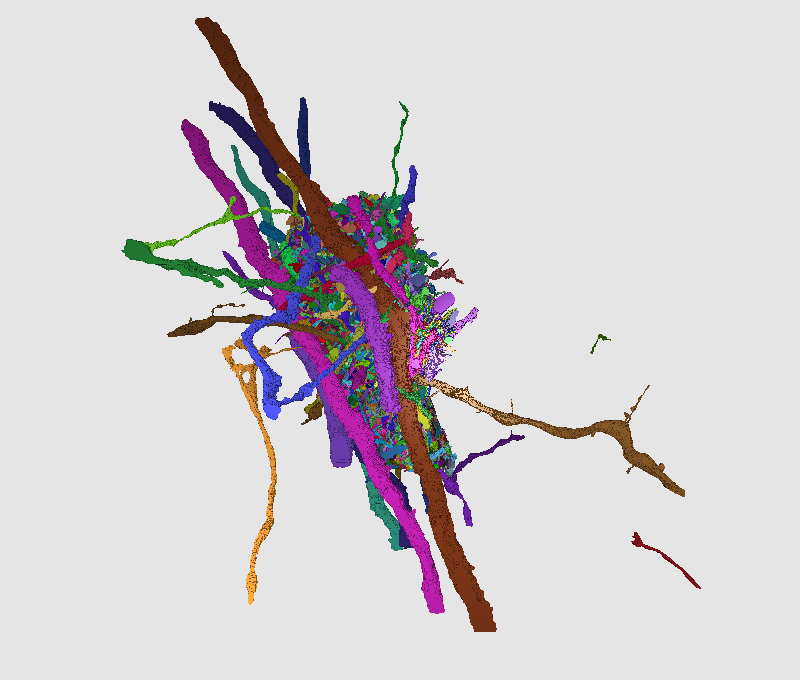
\includegraphics[width=\columnwidth]{figures/neurons_placeholder.png}
 \caption{Model of over 1600 neurons reconstructed from an electron microscopy scan of a mouse brain.}
 \label{fig:neurons}
\end{figure}

\begin{figure}[tb]
 \centering
 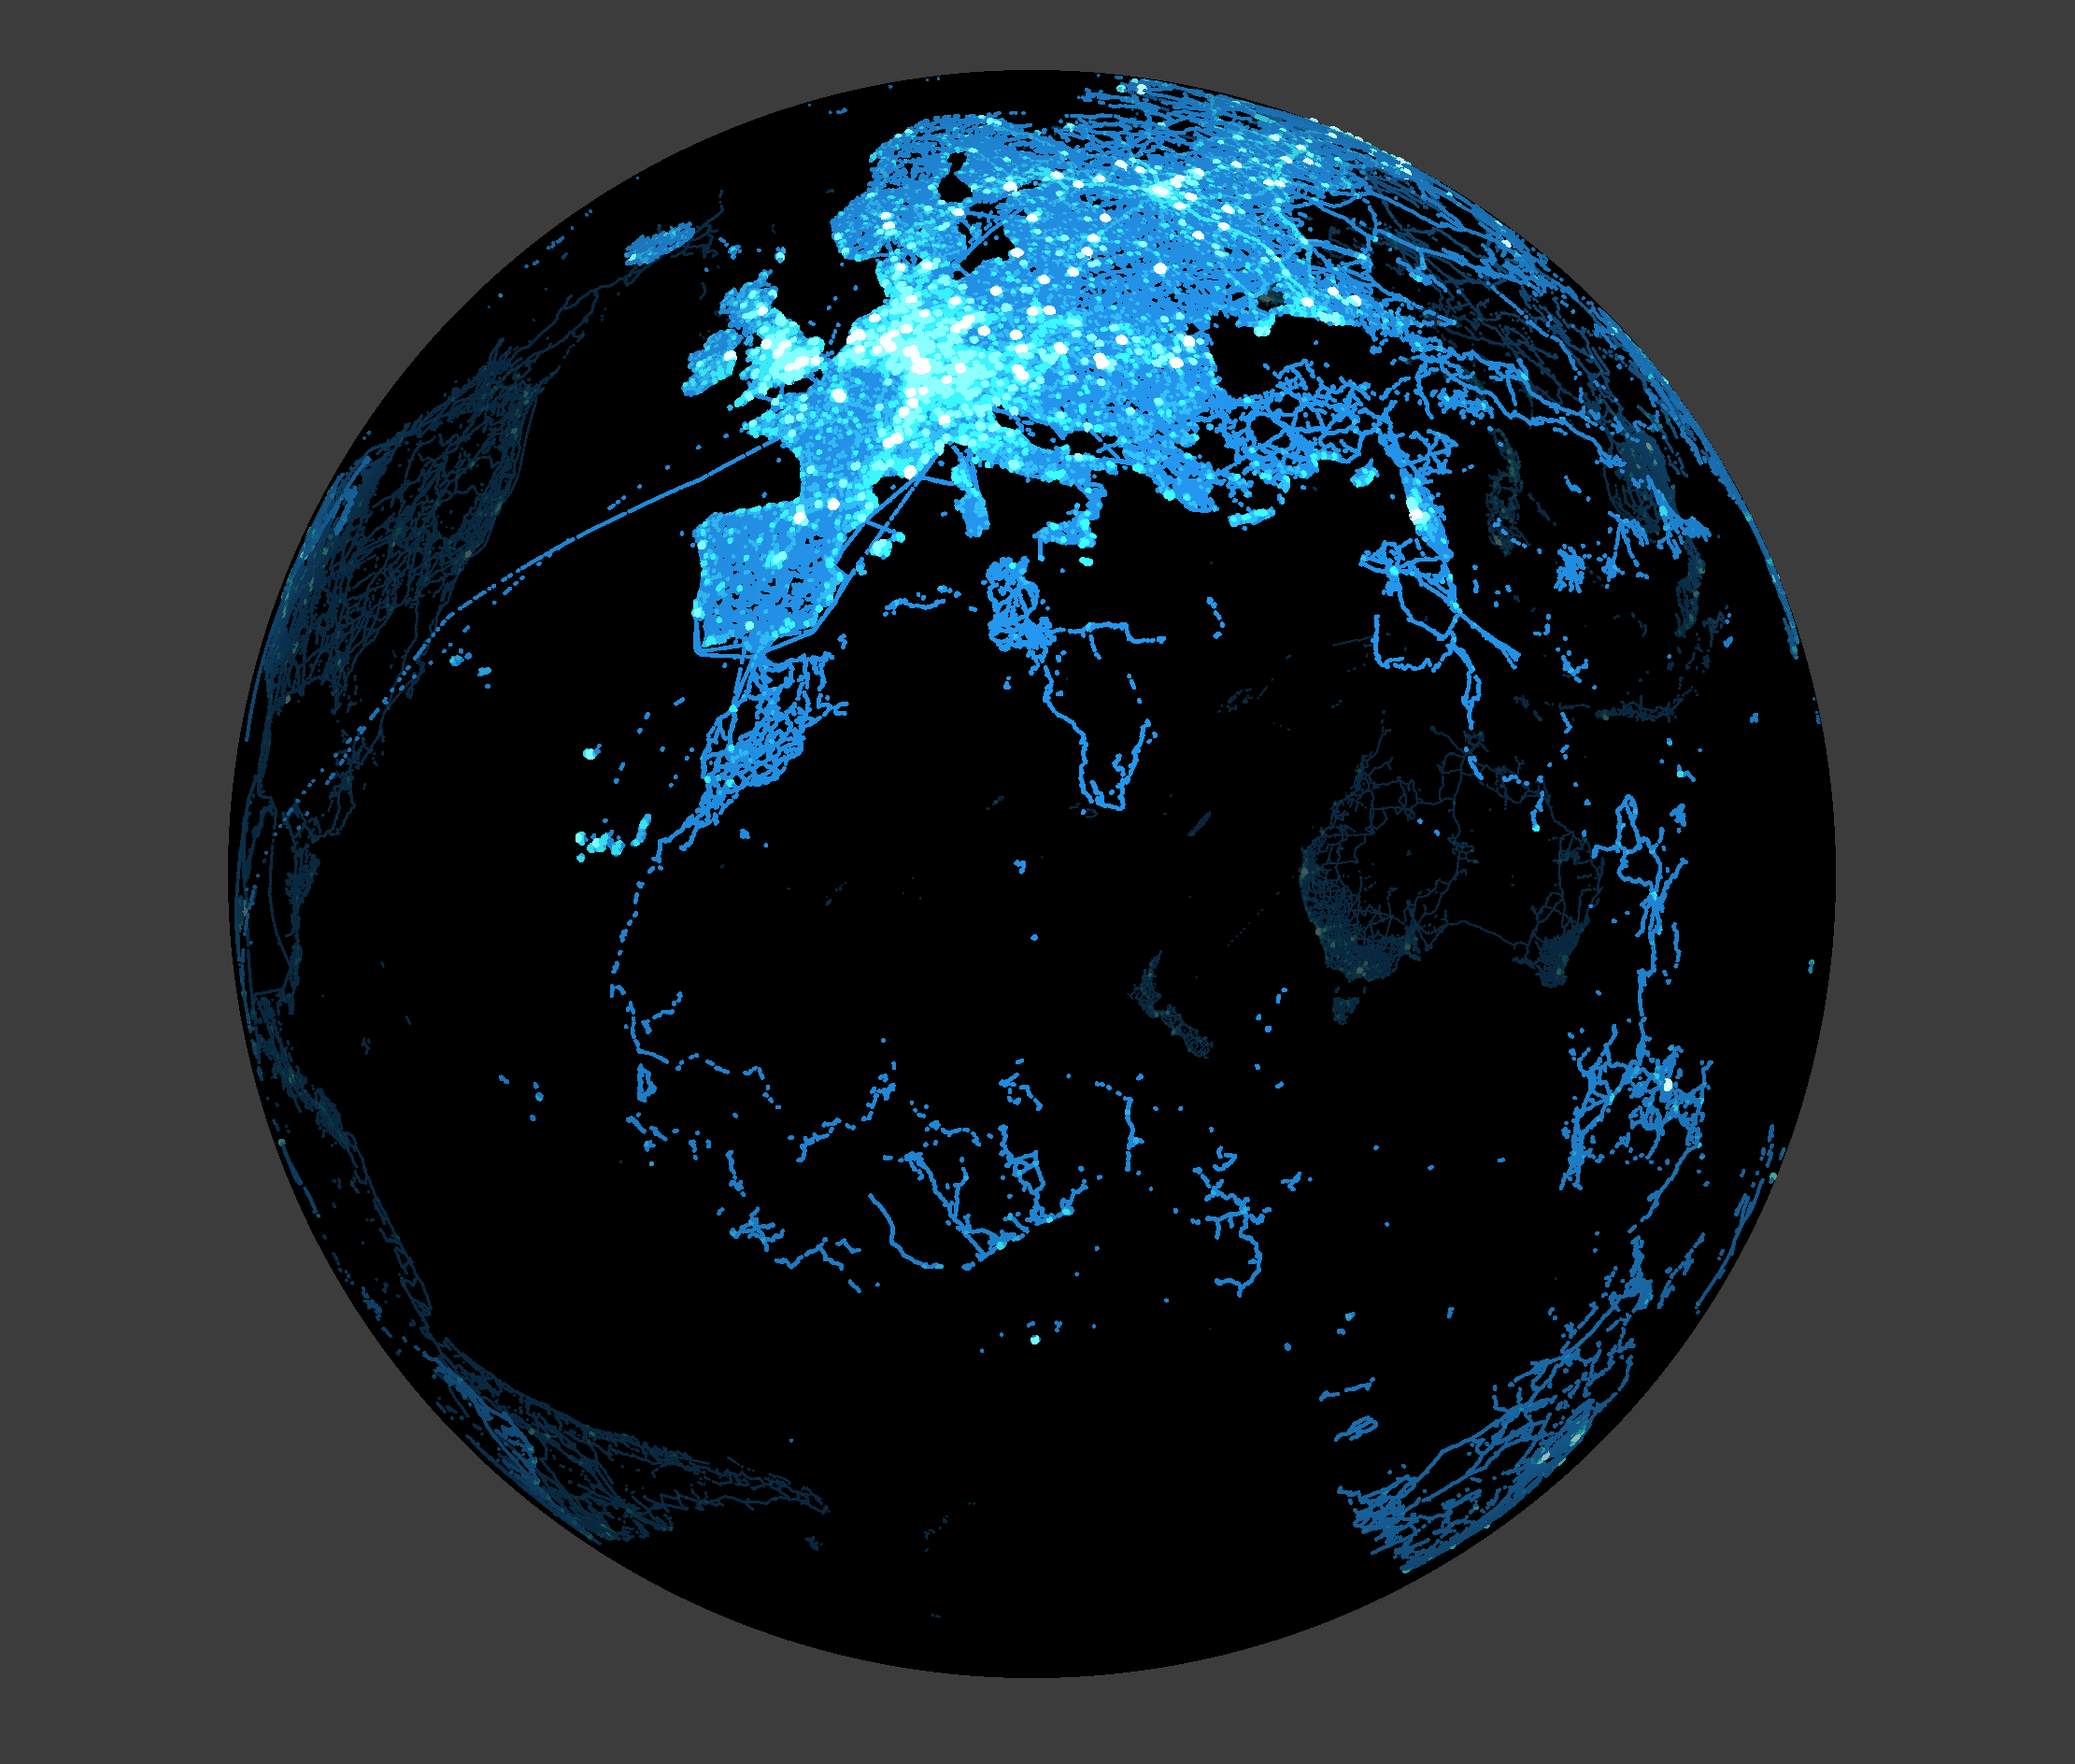
\includegraphics[width=\columnwidth]{figures/gps_55.3M.png}
 \caption{Point cloud of approximately 55.3 million GPS coordinates collected by OpenStreetMap.}
 \label{fig:gps}
\end{figure}

In order to evaluate the impact that performing Active Pixel encoding on the GPU has on distributed rendering applications, we measured both compute and memory transfer times as well as overall frame rate. We compared three of IceT's compositing methods: 1) generic compositing interface, 2) OpenGL 3 compositing interface, and 3) OpenGL 3 compositing interface with GPU compression. When using the generic compositing interface, the entire rendered framebuffer is provided to IceT and Active Pixel encoding occurs on the CPU. When using the OpenGL 3 compositing interface, region of interest detection is leveraged to reduce raw data memory transfer size, but Active Pixel encoding still occurs on the CPU. When using the OpenGL 3 compositing interface with GPU compression, Active Pixel encoding occurs on the GPU (taking into account the region of interest) and compressed image data is transferred to main memory.

It is also worth noting that rendering with IceT's generic interface can be configured to use region of interest detection. However, we wanted to be able to measure the relative benefit of GPU-based compression compared to that of region of interest detection. Additionally, we feel that the burden of configuring region of interest detection using the generic compositing interface is non-negligible and therefore application developers may not implement it in their distributed rendering applications.

We used three different data sets in our experiments -- a simple model of a nuclear power station, reconstructed neurons from an electron microscopy scan of a mouse brain, and latitude/longitude coordinates collected from GPS devices by OpenStreetMap (shown in Figs. \ref{fig:intro}, \ref{fig:neurons}, and \ref{fig:gps} respectively). The nuclear power station is stored as 34 separate OBJ files and contains 9,096 triangles in total. The neuron data set is stored as 1632 separate OBJ files and contains just over 91 million triangles in total. The GPS data set contains approximately 2.77 billion latitude/longitude coordinates, of which 2\% were preprocessed for use with our experiments. The resulting \textapprox{}55.3 million latitude/longitude coordinates were mapped onto a globe in 3D and rendered using an imposter sphere point cloud visualization with both size and color mapped to density.

For each data set and compositing method, we performed strong scaling tests at three different resolutions -- HD ($1920\times1080$), 4K ($3840\times2160$), and 8K ($7680\times4320$). For the nuclear power station and neuron data sets, OBJ files were distributed amongst rendering processes. For the GPS data set, points were distributed based on latitude/longitude with an equal number of points per process. The nuclear power station data set was rendered using 2, 4, 8, 16, and 32 processes. The neuron and GPS data sets were rendered using 6, 12, 24, 48, 96, and 192 processes.

\begin{figure*}[!b]
  \centering % avoid the use of \begin{center}...\end{center} and use \centering instead (more compact)
  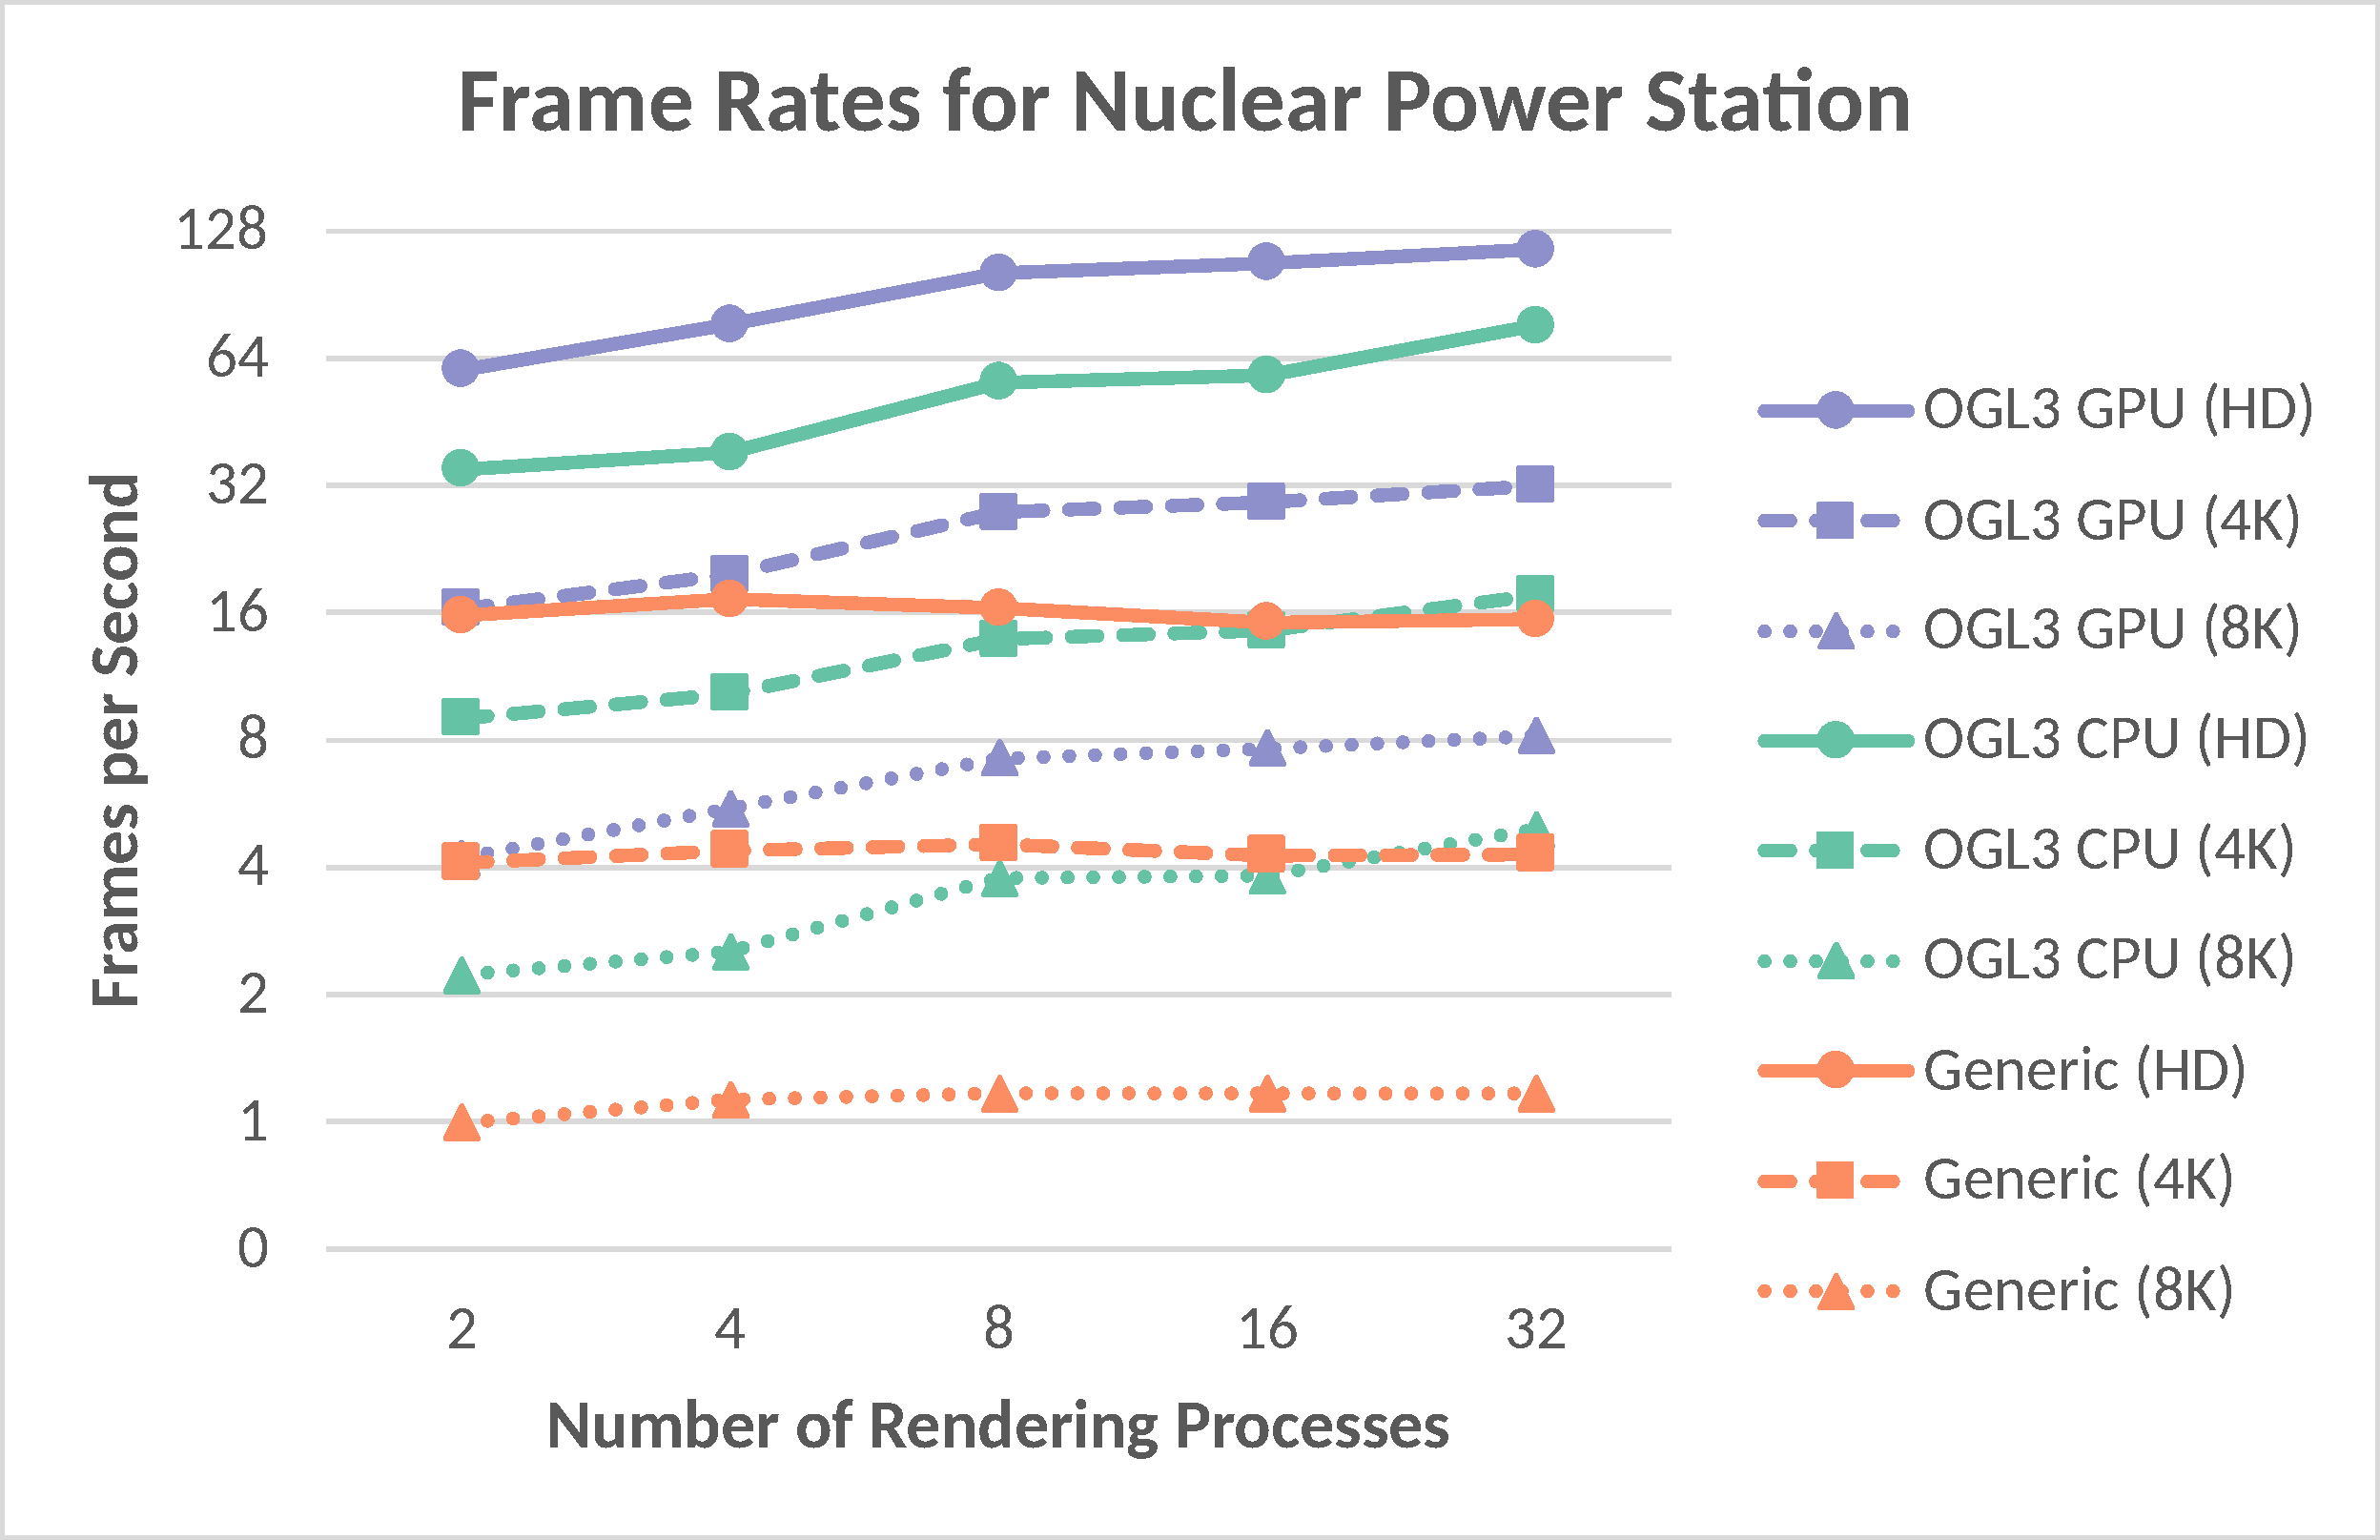
\includegraphics[width=0.494\textwidth,page=1]{FPS_NuclearPowerStation.pdf}
  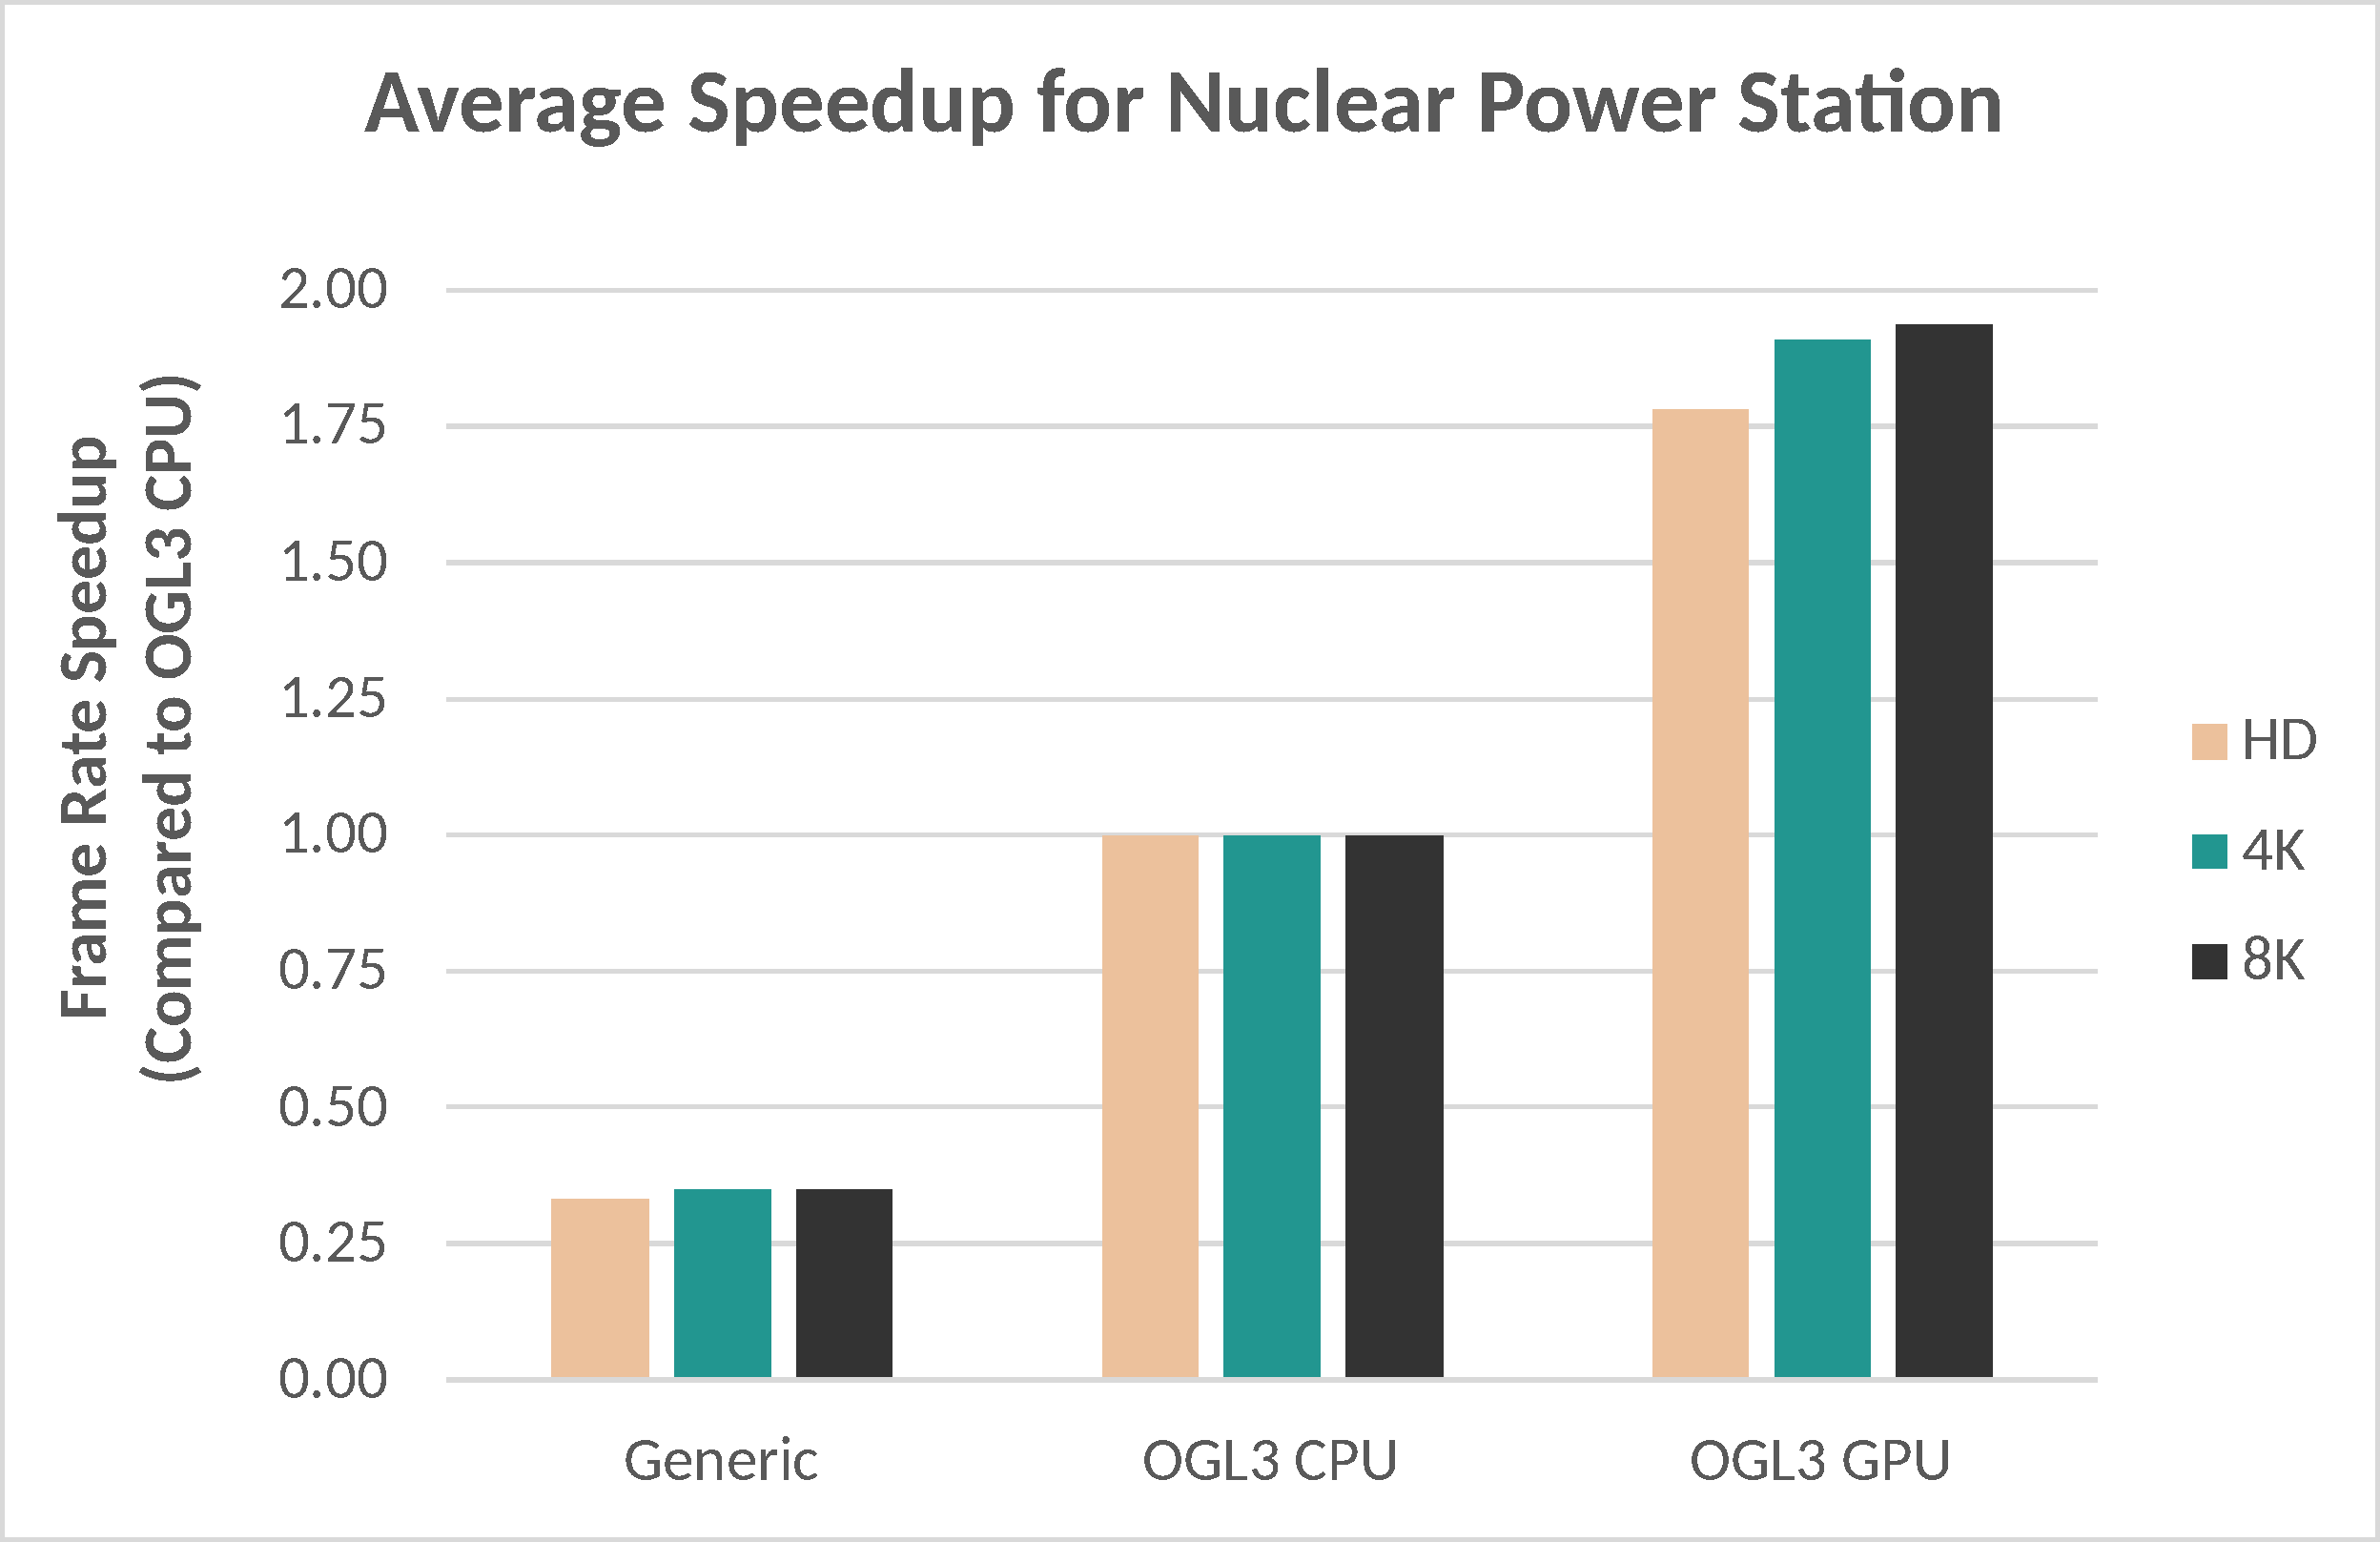
\includegraphics[width=0.494\textwidth,page=1]{Speedup_NuclearPowerStation.pdf}\\
  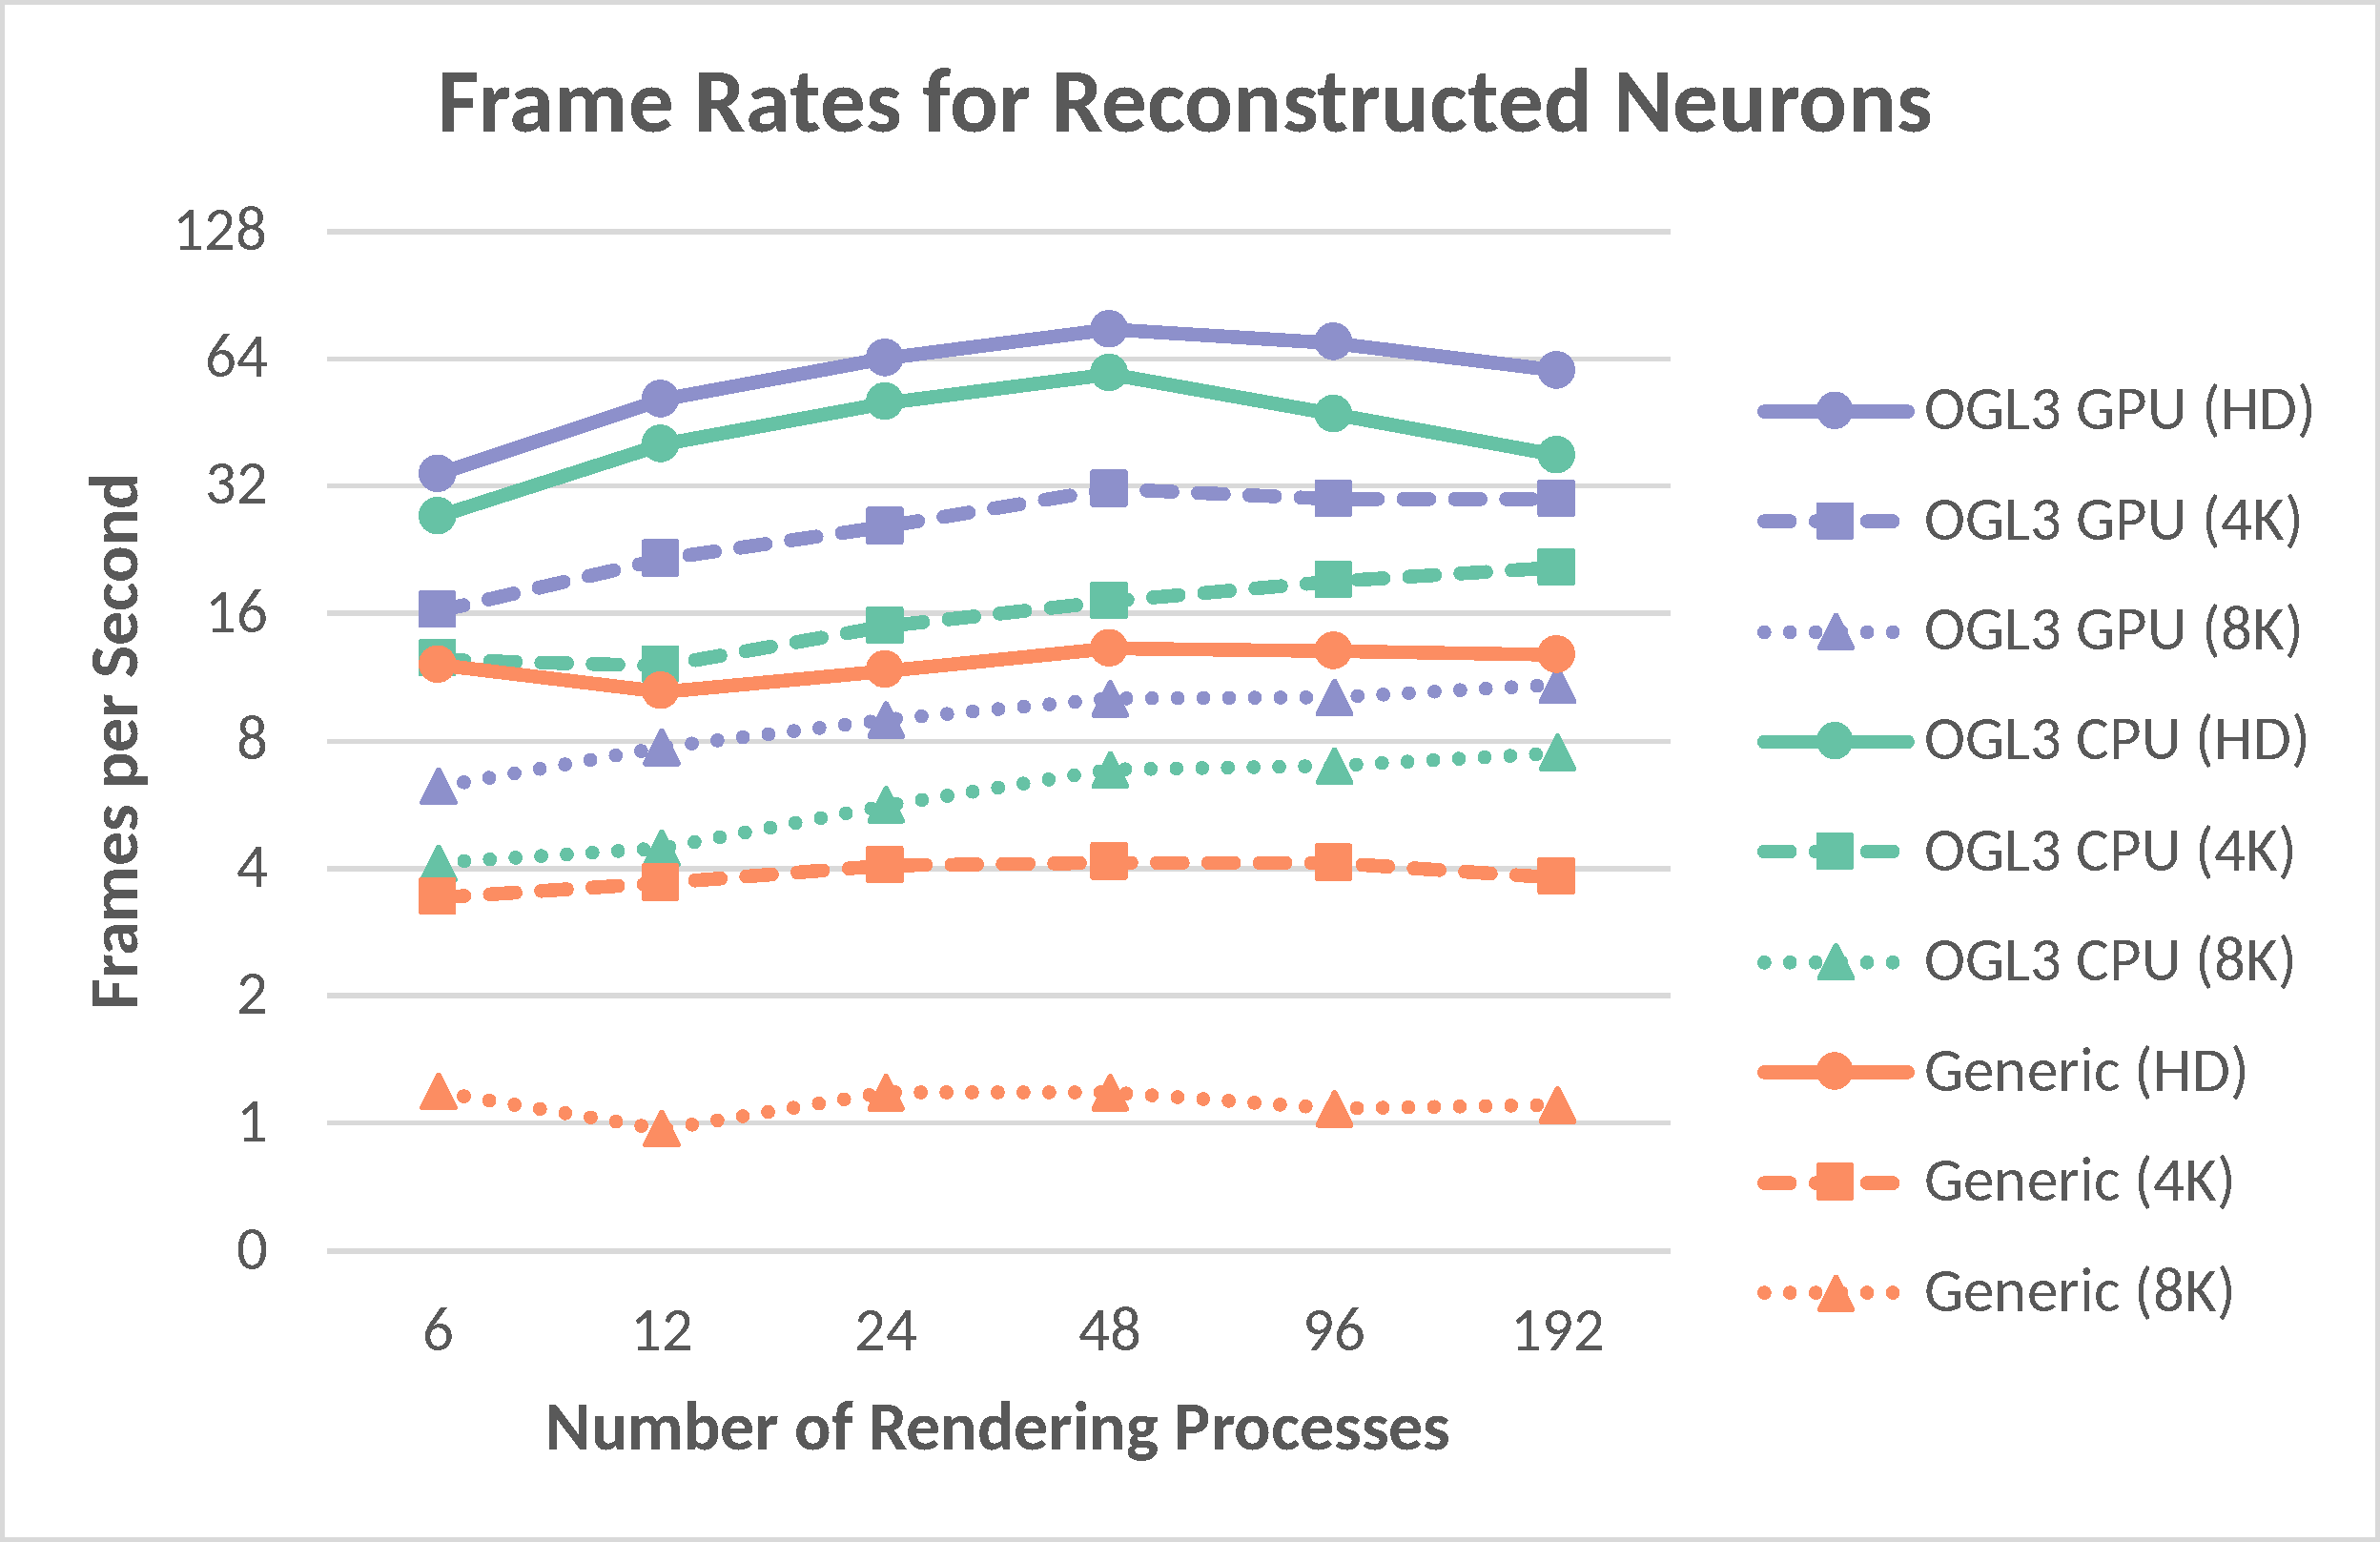
\includegraphics[width=0.494\textwidth,page=1]{FPS_ReconstructedNeurons.pdf}
  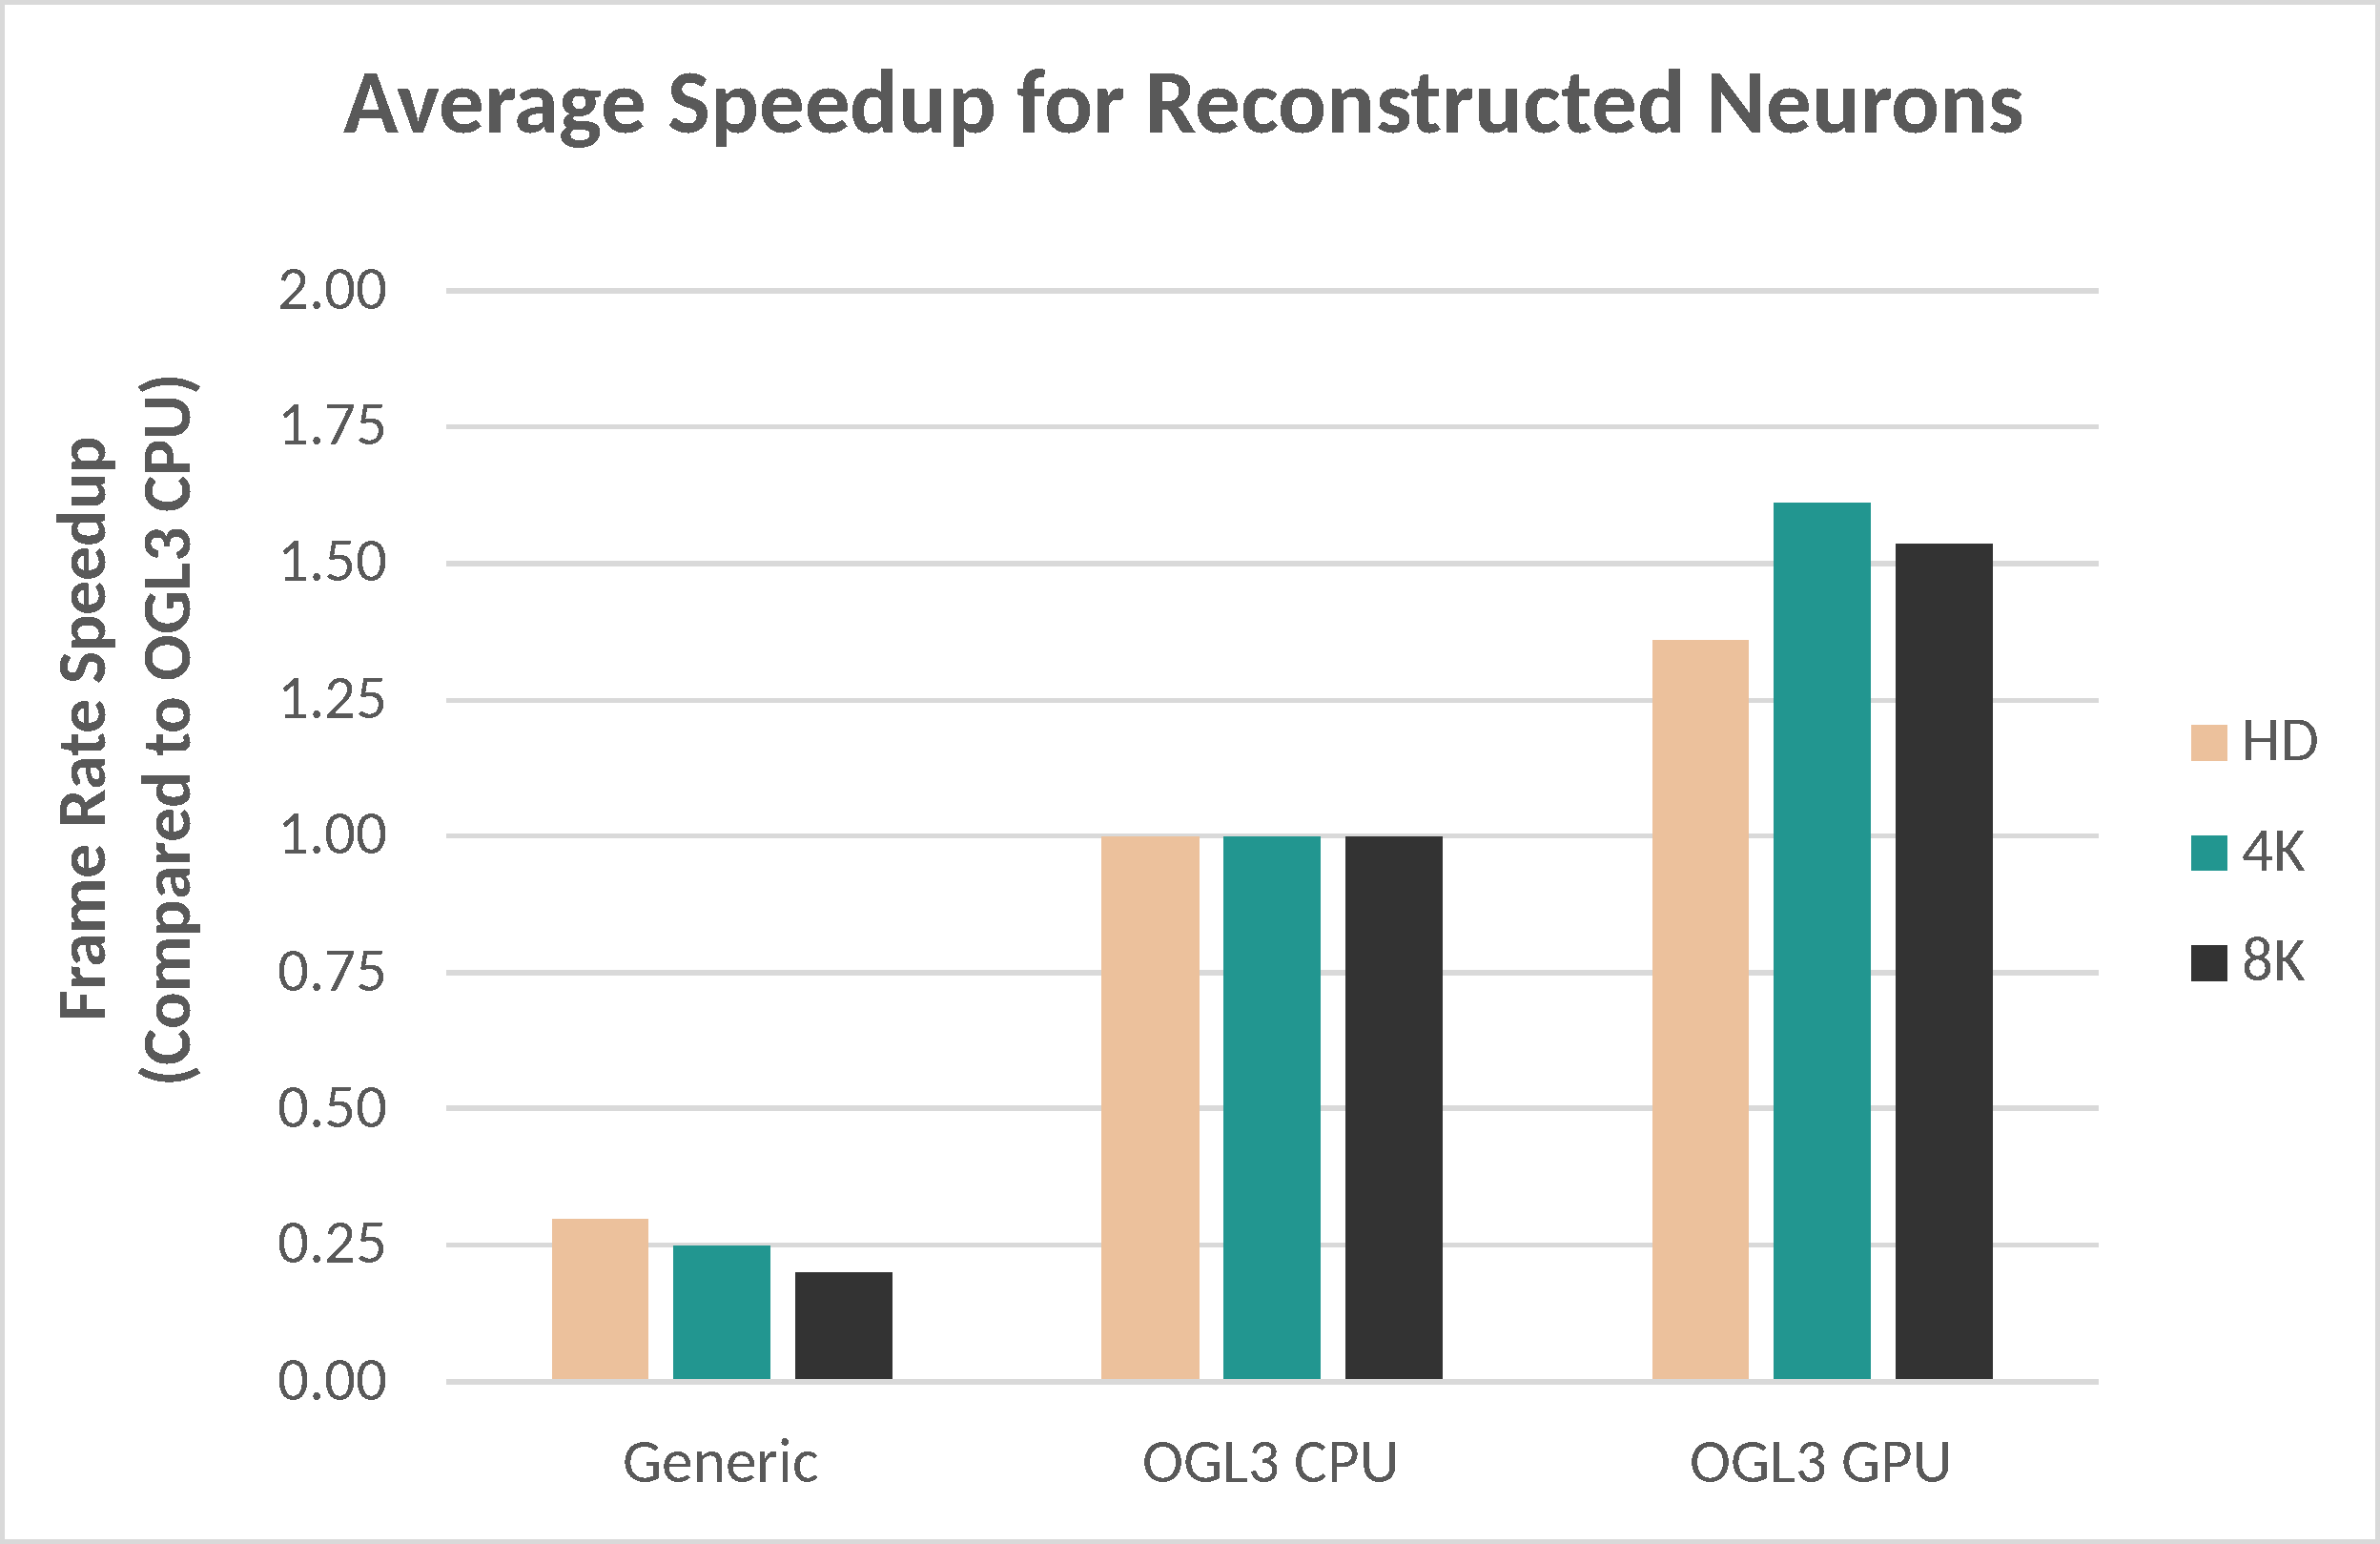
\includegraphics[width=0.494\textwidth,page=1]{Speedup_ReconstructedNeurons.pdf}\\
  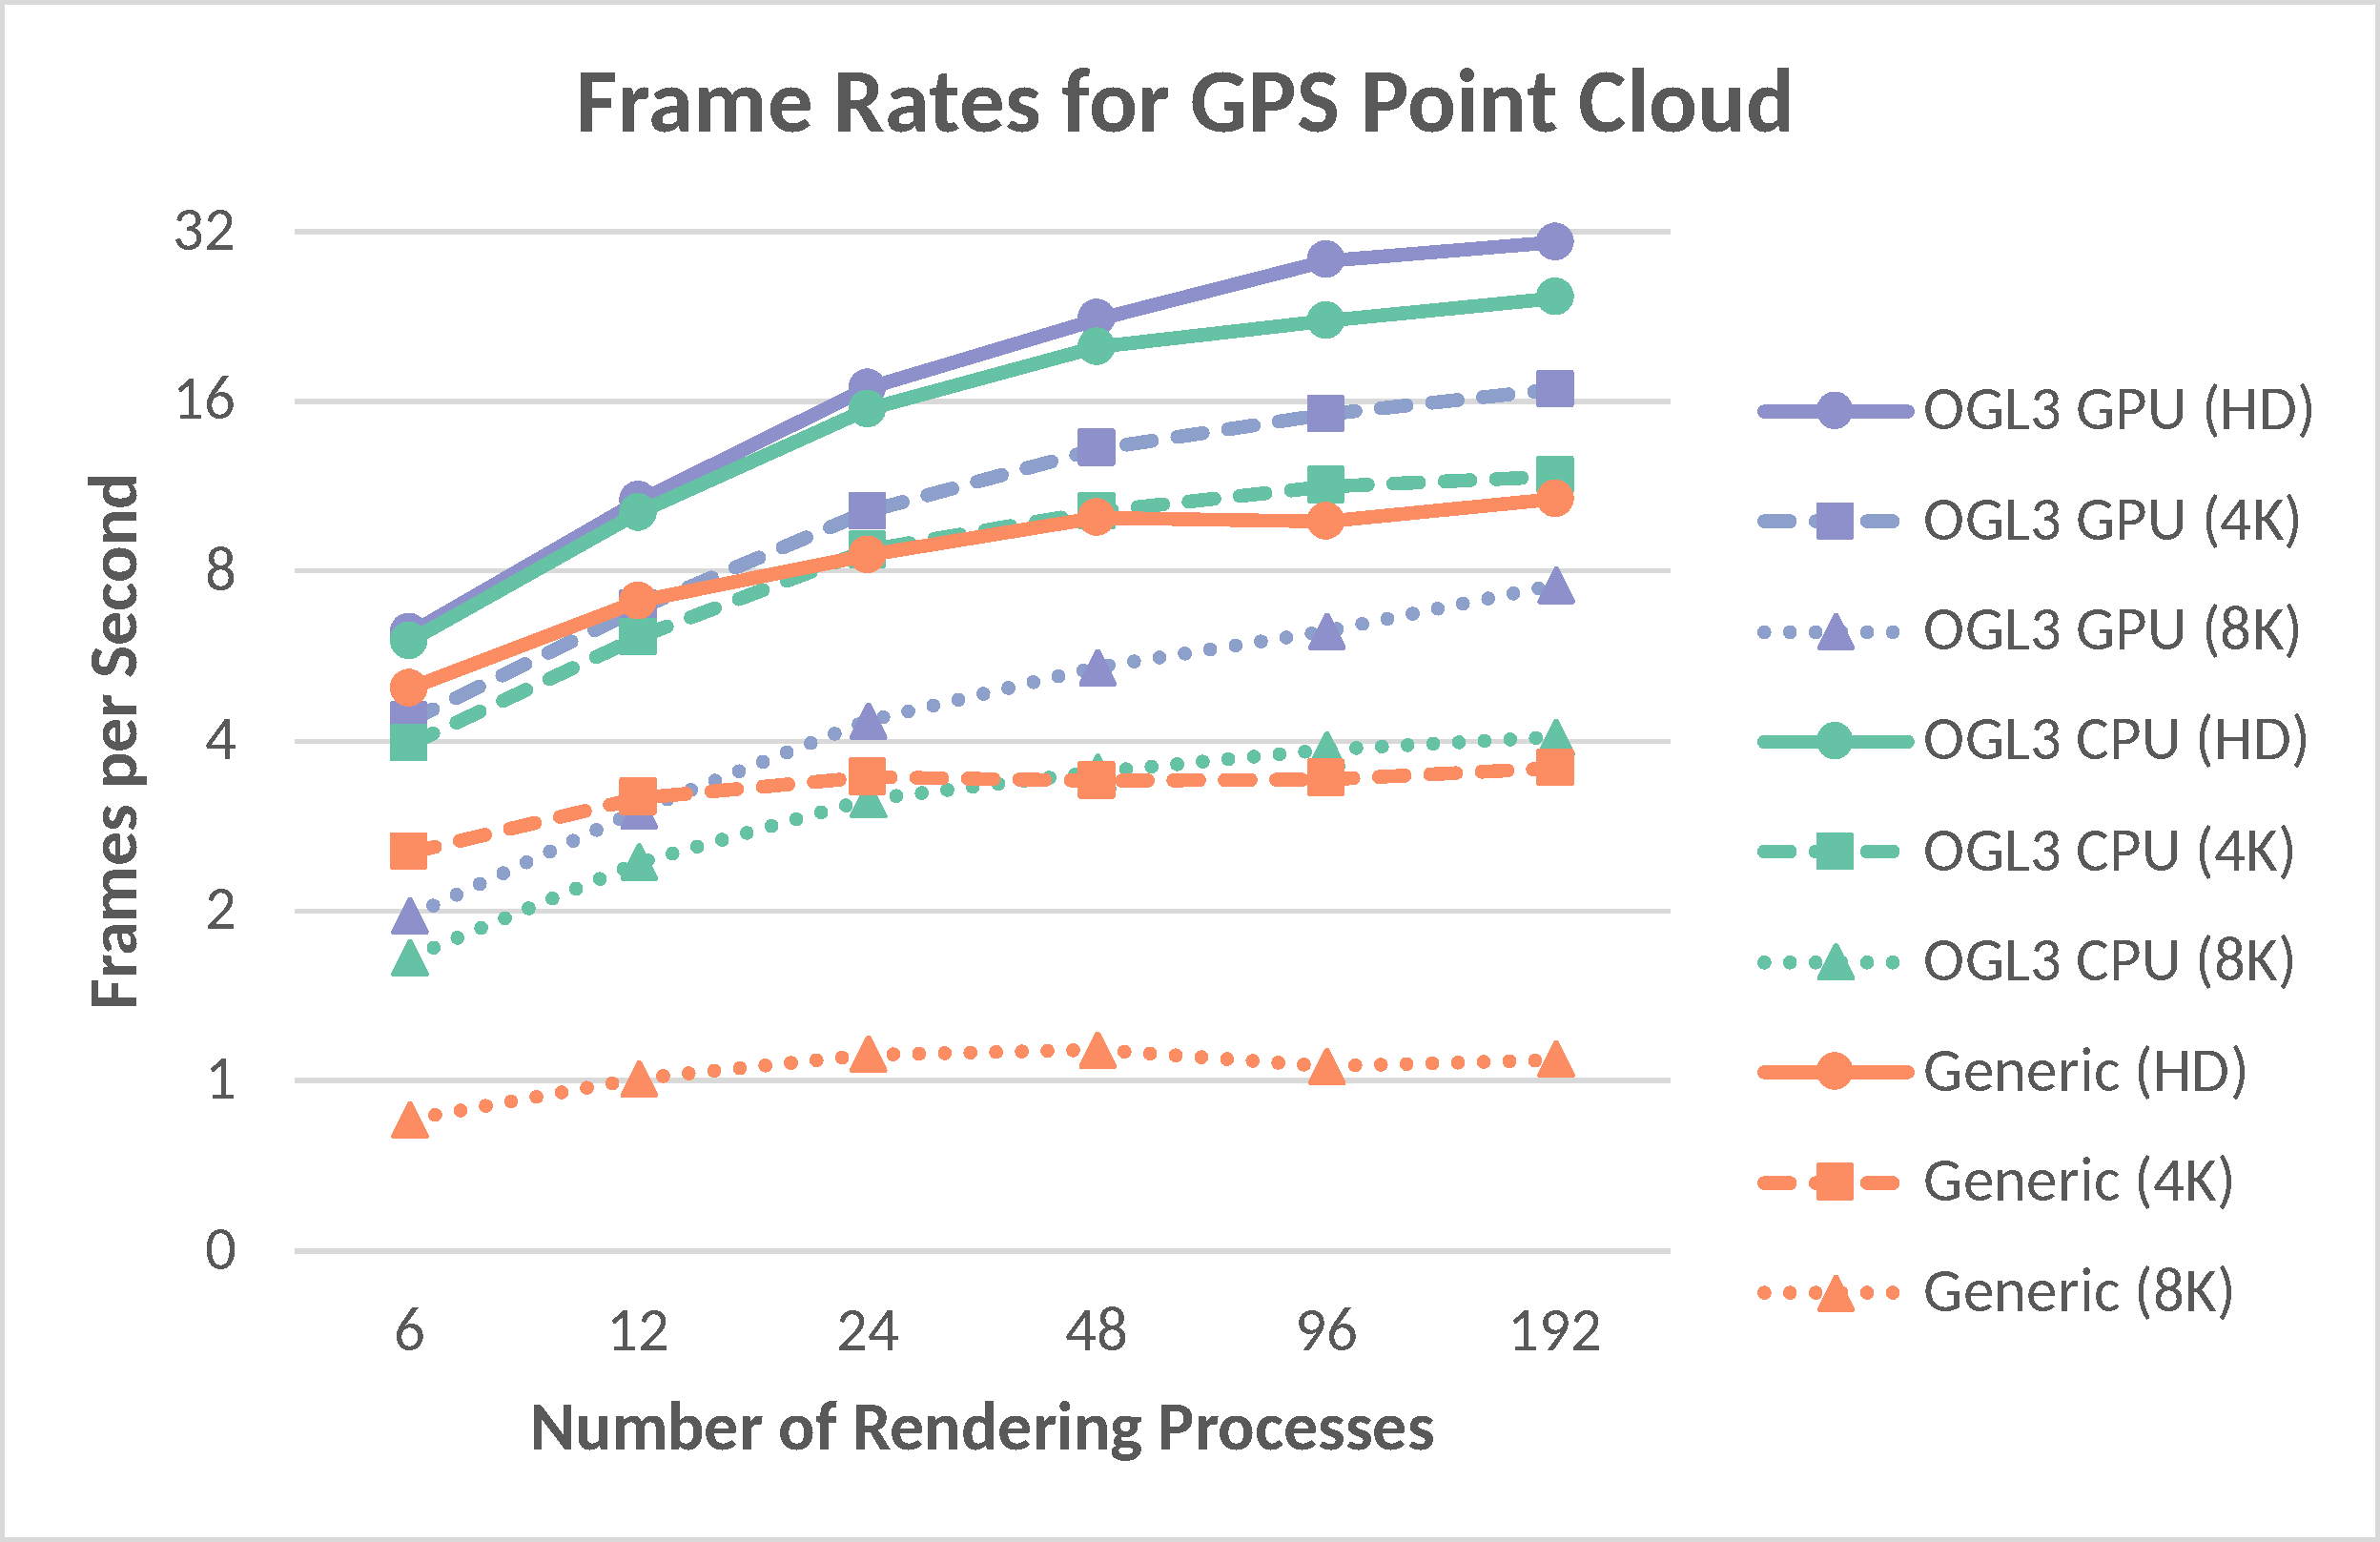
\includegraphics[width=0.494\textwidth,page=1]{FPS_GPSPointCloud.pdf}
  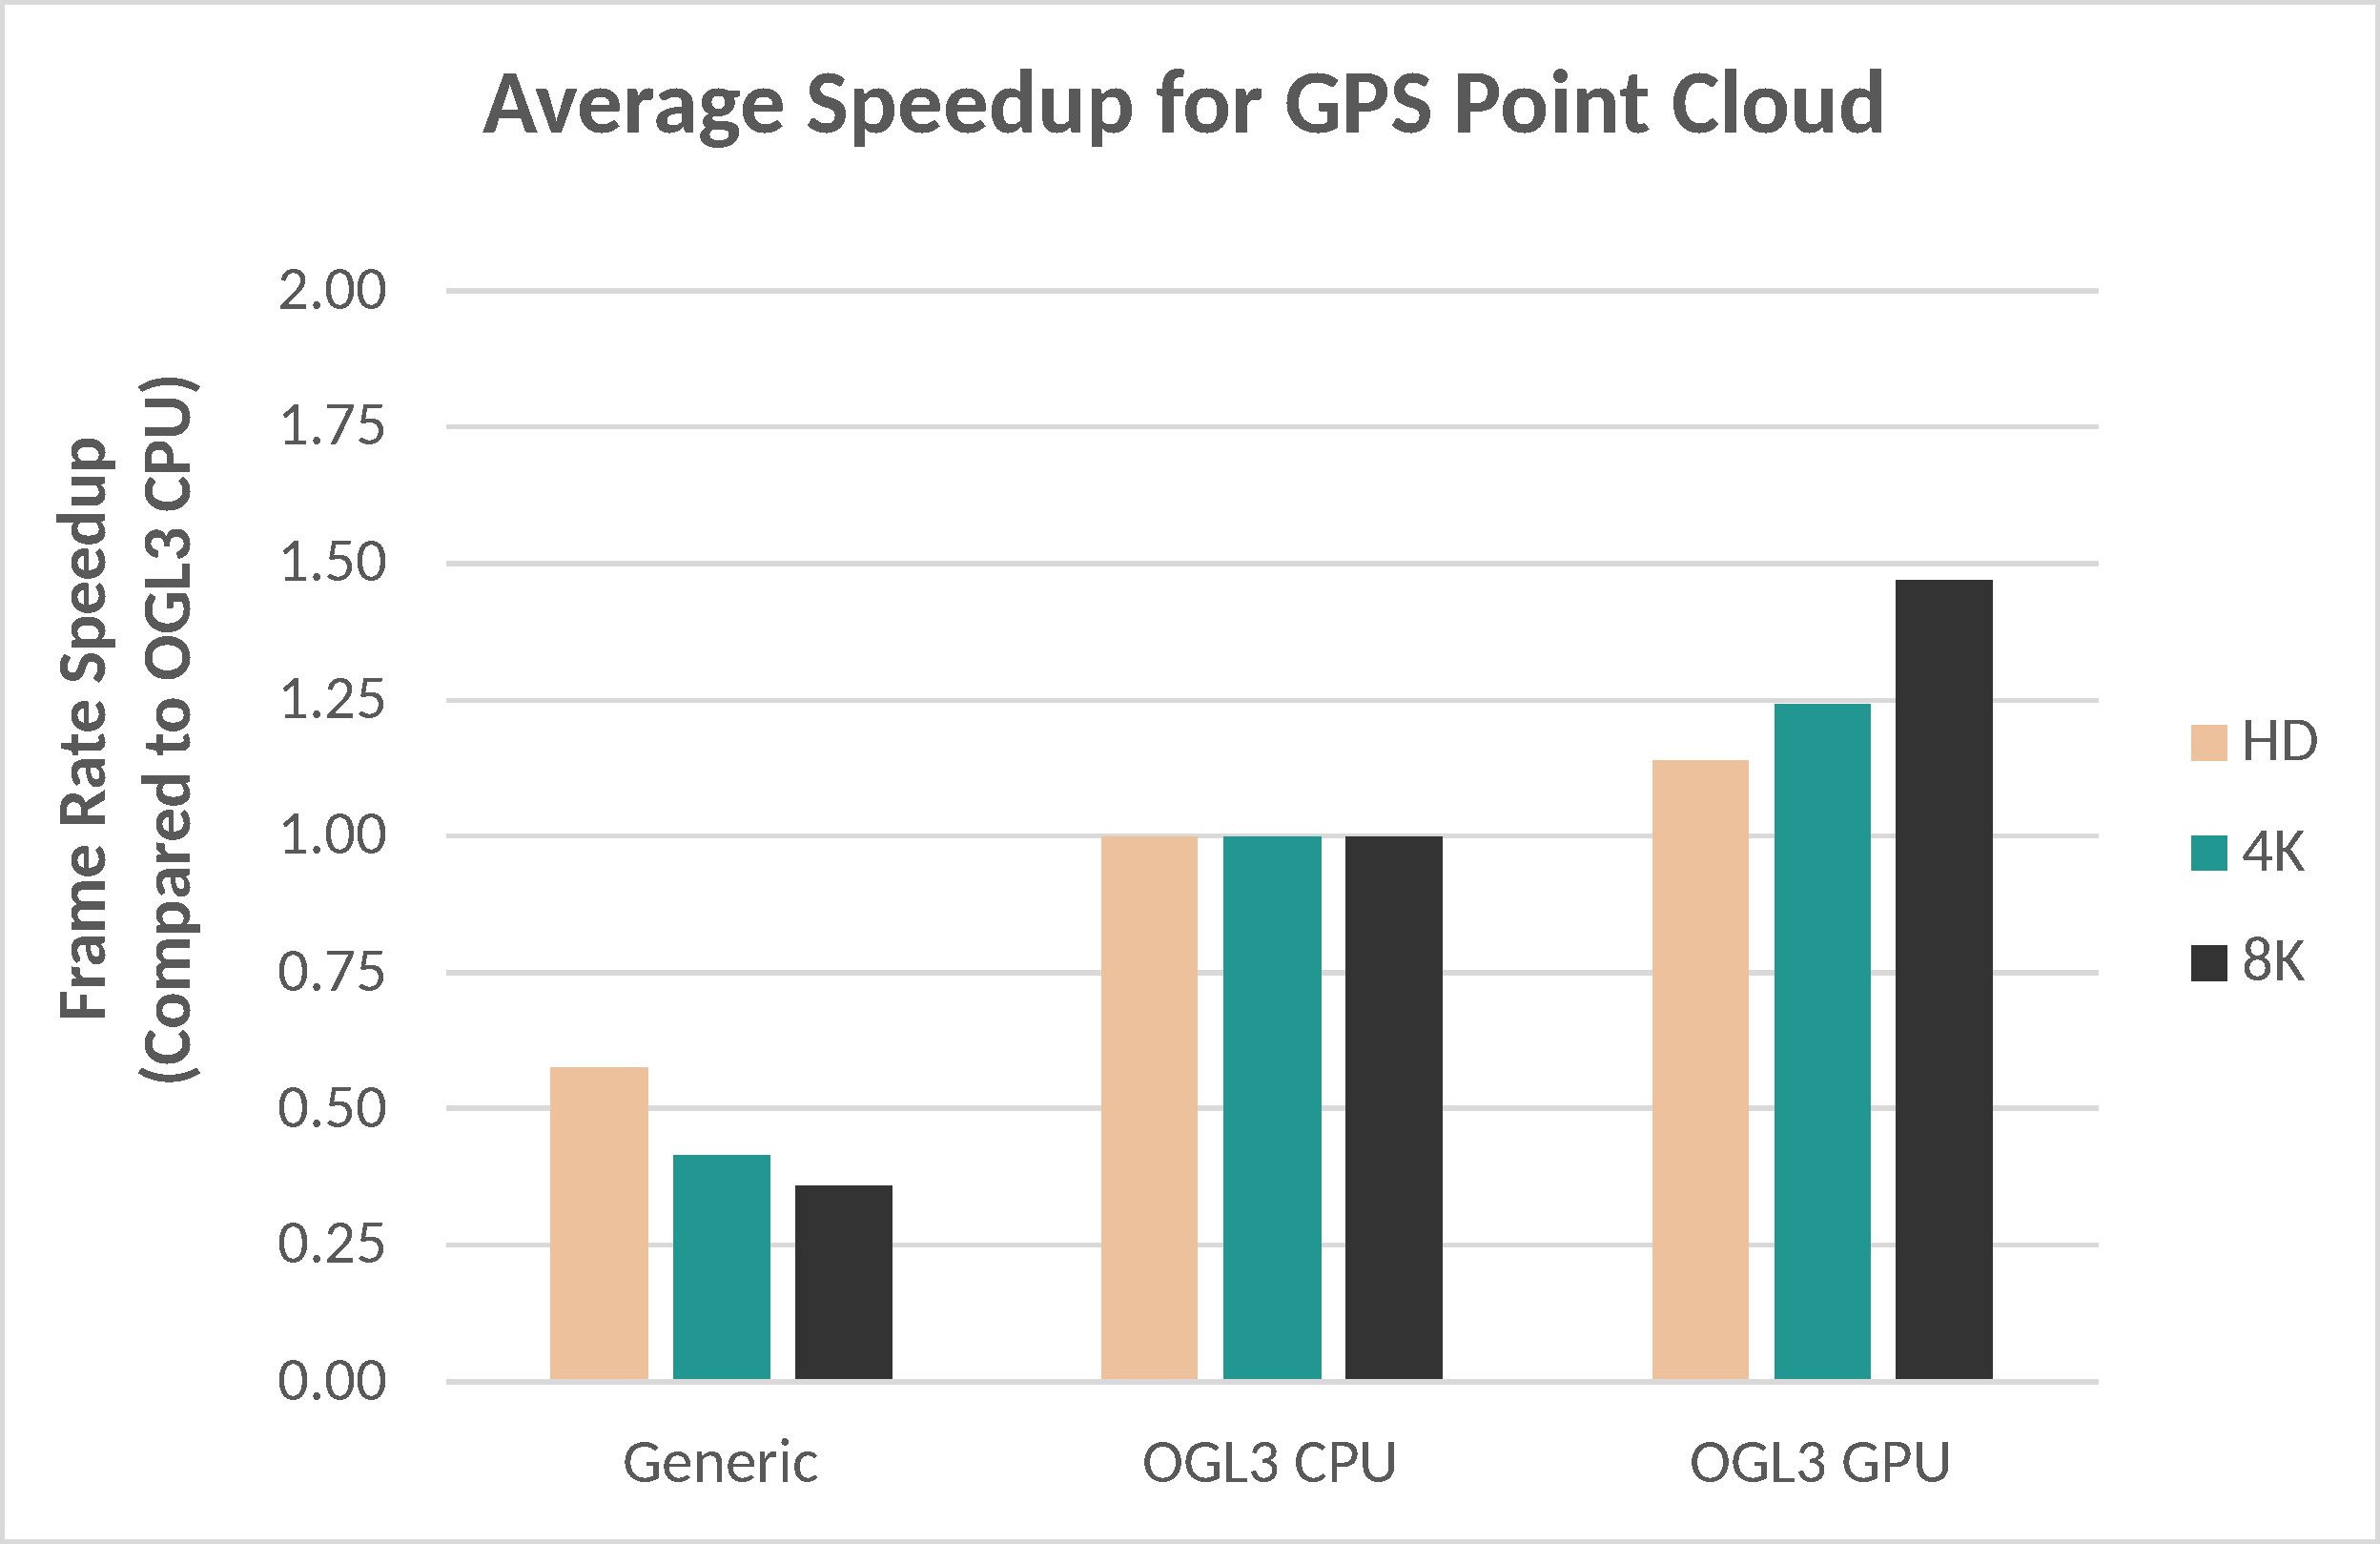
\includegraphics[width=0.494\textwidth,page=1]{Speedup_GPSPointCloud.pdf}
  \caption{Frame rate results for nuclear power station, reconstructed neurons, and GPS point cloud data sets rendered at HD, 4K, and 8K using the three compositing techniques. Left column shows strong scaling results when measuring overall frames per second. Right column shows relative frame rate speed (with the regular OpenGL 3 compositing interface as the reference).}
  \label{fig:results_fps}
\end{figure*}

The nuclear power station data set intentionally has a low polygon count, which leads to quick render times even with a small number of processes. This results in compositing as the main bottleneck in the distributed rendering pipeline. The neuron and GPS data sets are intentionally larger-scale. When using a small number of processes, data is either too large to fit in GPU memory or leads to non-interactive render times. However, when using a large number of processes, data easily fits in GPU memory and can be rendered quickly. Therefore, as more processes are used, these distributed rendering applications move from having rendering as their bottleneck to having compositing as their bottleneck.

All tests were run on Argonne National Laboratory's Cooley system -- a 126-node cluster with an NVIDIA Tesla K80 dual GPU in each node and a 56 Gbps FDR InfiniBand interconnect. Each test used two processes per node (with each using a separate GPU). Visualizations of each data set positioned the models to fill the center of the screen. The models were rotated 360\textdegree{} over 180 frames. Our main goal was to speed up the overall distributed rendering pipeline. Therefore the primary dependent variable we were interested in observing was frame rate, measured in average frames per second (FPS). Secondarily, we also were interested in observing compression compute time and device-to-host data transfer time.

\subsection{Frame Rate Comparison}
\setlength{\tabcolsep}{0.44em} % for the horizontal padding
\begin{table*}[!hb]
\centering
\caption{Timing results for performing GPU to main memory image transfer and computation for image compression. Results from smallest scale runs shown in blue. Results from largest scale runs shown in red.}
\begin{tabular}{ |l|c;{2pt/2pt}c|c;{2pt/2pt}c|c;{2pt/2pt}c|c;{2pt/2pt}c|c;{2pt/2pt}c|c;{2pt/2pt}c| }
 \hline
 & \multicolumn{4}{c|}{\textbf{Nuclear Power Station}} & \multicolumn{4}{c|}{\textbf{Reconstructed Neurons}} & \multicolumn{4}{c|}{\textbf{GPS Point Cloud}} \\
 & \multicolumn{2}{c}{Mem. Transfer} & \multicolumn{2}{c|}{Compression} & \multicolumn{2}{c}{Mem. Transfer} & \multicolumn{2}{c|}{Compression} & \multicolumn{2}{c}{Mem. Transfer} & \multicolumn{2}{c|}{Compression} \\
 & \multicolumn{2}{c}{(milliseconds)} & \multicolumn{2}{c|}{(milliseconds)} & \multicolumn{2}{c}{(milliseconds)} & \multicolumn{2}{c|}{(milliseconds)} & \multicolumn{2}{c}{(milliseconds)} & \multicolumn{2}{c|}{(milliseconds)} \\
 \hline
 
 \makecell[l]{\textbf{HD} ($1920\times1080$)} & \multicolumn{12}{c|}{ } \\\cline{2-13}
 \makecell[l]{\hspace*{4mm}Generic} & \color{small_scale}39.518 & \color{large_scale}41.536 & \color{small_scale}6.790 & \color{large_scale}5.922 & \color{small_scale}38.228 & \color{large_scale}41.631 & \color{small_scale}6.080 & \color{large_scale}5.920 & \color{small_scale}36.539 & \color{large_scale}43.184 & \color{small_scale}6.172 & \color{large_scale}5.877 \\
 \makecell[l]{\hspace*{4mm}OGL3 CPU} & \color{small_scale}6.819 & \color{large_scale}0.488 & \color{small_scale}4.344 & \color{large_scale}0.259 & \color{small_scale}2.535 & \color{large_scale}0.689 & \color{small_scale}1.388 & \color{large_scale}0.280 & \color{small_scale}4.140 & \color{large_scale}2.256 & \color{small_scale}2.584 & \color{large_scale}0.964 \\
 \makecell[l]{\hspace*{4mm}OGL3 GPU} & \color{small_scale}0.358 & \color{large_scale}0.048 & \color{small_scale}1.072 & \color{large_scale}0.495 & \color{small_scale}0.066 & \color{large_scale}0.029 & \color{small_scale}0.712 & \color{large_scale}0.642 & \color{small_scale}0.044 & \color{large_scale}0.027 & \color{small_scale}0.689 & \color{large_scale}0.719 \\
 \hline
 
 \makecell[l]{\textbf{4K} ($3840\times2160$)} & \multicolumn{12}{c|}{ } \\\cline{2-13}
 \makecell[l]{\hspace*{4mm}Generic} & \color{small_scale}152.554 & \color{large_scale}158.988 & \color{small_scale}26.992 & \color{large_scale}23.724 & \color{small_scale}156.545 & \color{large_scale}158.900 & \color{small_scale}24.224 & \color{large_scale}23.562 & \color{small_scale}143.465 & \color{large_scale}159.966 & \color{small_scale}24.118 & \color{large_scale}23.466 \\
 \makecell[l]{\hspace*{4mm}OGL3 CPU} & \color{small_scale}22.826 & \color{large_scale}1.574 & \color{small_scale}17.289 & \color{large_scale}1.004 & \color{small_scale}8.347 & \color{large_scale}2.080 & \color{small_scale}5.404 & \color{large_scale}1.011 & \color{small_scale}15.602 & \color{large_scale}7.835 & \color{small_scale}9.994 & \color{large_scale}3.811 \\
 \makecell[l]{\hspace*{4mm}OGL3 GPU} & \color{small_scale}1.261 & \color{large_scale}0.120 & \color{small_scale}2.768 & \color{large_scale}0.819 & \color{small_scale}0.253 & \color{large_scale}0.042 & \color{small_scale}2.522 & \color{large_scale}1.379 & \color{small_scale}0.097 & \color{large_scale}0.031 & \color{small_scale}1.809 & \color{large_scale}1.717 \\
 \hline
 
 \makecell[l]{\textbf{8K} ($7680\times4320$)} & \multicolumn{12}{c|}{ } \\\cline{2-13}
 \makecell[l]{\hspace*{4mm}Generic} & \color{small_scale}658.877 & \color{large_scale}633.736 & \color{small_scale}108.929 & \color{large_scale}95.005 & \color{small_scale}591.419 & \color{large_scale}632.637 & \color{small_scale}96.580 & \color{large_scale}94.081 & \color{small_scale}574.176 & \color{large_scale}632.394 & \color{small_scale}96.198 & \color{large_scale}93.711 \\
 \makecell[l]{\hspace*{4mm}OGL3 CPU} & \color{small_scale}105.717 & \color{large_scale}5.816 & \color{small_scale}69.041 & \color{large_scale}4.048 & \color{small_scale}32.841 & \color{large_scale}7.046 & \color{small_scale}21.055 & \color{large_scale}3.879 & \color{small_scale}61.075 & \color{large_scale}29.594 & \color{small_scale}39.376 & \color{large_scale}15.239 \\
 \makecell[l]{\hspace*{4mm}OGL3 GPU} & \color{small_scale}5.764 & \color{large_scale}0.410 & \color{small_scale}10.818 & \color{large_scale}2.114 & \color{small_scale}0.930 & \color{large_scale}0.092 & \color{small_scale}8.853 & \color{large_scale}4.292 & \color{small_scale}0.297 & \color{large_scale}0.043 & \color{small_scale}6.248 & \color{large_scale}5.669 \\
 \hline
\end{tabular}
\label{table:memtransfer_compression}
\end{table*}

The main goal of our work was to improve distributed rendering time, thus leading to higher frame rates. Results from rendering the nuclear power station, reconstructed neurons, and GPS point cloud data sets are visualized in the left column of \autoref{fig:results_fps}. The two compositing techniques using the new OpenGL 3 compositing interface for IceT were able to achieve substantially higher frame rates than the generic compositing interface, which falls in line with prior experiments showing that region of interest detection can greatly improve compositing efficiency. Additionally, the OpenGL 3 compositing interface with GPU-based compression resulted in achieving even higher frame rates than when performing the compression on the CPU. Results also show that the OpenGL 3 compositing interface with GPU-based compression scales better as the improved frame rates become more pronouced at higher process counts.

We observe that the frame rate for each data set plateaus (or even decreases) at some point. Adding processes benefits the distributed rendering pipeline by reducing the amount of geometry each process is responsible for rendering and shrinking the region of interest each process uses during compositing. However, extra processes also add more communication for the compositing step. As with any strong scaling setup, at some point the benefits of reduced computation are outweighed by increased overheads.

Our three data sets show three different behaviors. The nuclear power station receives almost no boost to rendering performance as the number of processes increase since there is so little geometry to begin with. Distributed rendering frame rates increase nonetheless for both compositing methods that use the OpenGL 3 interface due to the fact that the region of interest for each rendering process is shrinking. The reconstructed neurons also receives little to no boost in rendering performance as the number of processes increase. While this data set is larger, it is already being split into 6 parts at the smallest tested scale. We were however able to split the data amongst a higher number of processes and therefore observe the point when adding more rendering processes became detrimental to the overall performance of the application. The GPS point cloud applications shows nice scaling as the number of rendering processes increase. Even the generic compositing interface (which does not use region of interest detection) sees an increase in frame rate as the application uses more rendering processes. However, this application also sees diminishing returns after a certain point, with frame rates typically only slightly increasing between the largest two runs.

In addition to looking at raw frame rates, we compared average frame rates across all scales to the regular OpenGL 3 compositing interface for each data set / resolution combination. This metric gave us an average distributed rendering speedup achieved by each compositing technique when compared to the prior state-of-the-art of using region of interest detection, but copying raw pixels off the GPU and performing compression on the CPU. Results for the nuclear power station, reconstructed neurons, and GPS point cloud data sets are visualized in the right column of \autoref{fig:results_fps}. Beyond the fact the using GPU-based compression led to a speed up of 1.1x-1.9x for the whole distributed rendering process, it is worth noting that the benefits typically became more pronounced as resolution increased. This is likely due to the fact that for our test applications rendering time is primarily impacted by geometry, not resolution. However, compositing time is primarily impacted by resolution, not geometry. Therefore, as image resolution increases, a larger portion of the distributed rendering pipeline is spent in the compositing phase, thus making the GPU-based compression approach more impactful.

\subsection{Data Transfer and Compression Time Comparison}
In order further investigate the impact that compositing technique has on distributed rendering applications, we compared GPU to main memory image transfer time and computation time for performing the Active Pixel compression. \autoref{table:memtransfer_compression} shows results for the nuclear power station, reconstructed neurons, and GPS point cloud data sets when run using a small number of rendering processes (2, 6, and 6 respectively) and a large number of rendering processes (32, 192, and 192 respectively).

Results show that region of interest detection can lead to a substantial decrease in both memory transfer time and compression computation time. When comparing the regular OpenGL 3 compositing interface to the generic compositing interface across all data sets and resolutions, the regular OpenGL 3 compositing interface led to a 5.8x-18.8x reduction in memory transfer time at small scale and a 19.1x-109.0x reduction in memory transfer time at large scale. It also led to a 1.6x-4.6x reduction in compression computation time at small scale and a 6.1x-24.3x reduction in compression computation time at large scale.

We note that the gains of using the regular OpenGL 3 compositing interface over the generic compositing interface are more substantial at large scale. This is due to the fact that the regular OpenGL 3 compositing interface uses region of interest detection whereas the generic compositing interface always uses the entire rendered image. As more rendering processes are used, each process is responsible for rendering less geometry, and therefore the region of interest is likely to shrink. The smaller the region of interest, the less data there is to transfer and the fewer pixels there are to compress.

Results also show that performing compression on the GPU can lead to a substantial decrease in both memory transfer time and compression computation time. When comparing the OpenGL 3 compositing interface with GPU-based compression to the regular OpenGL 3 compositing interface across all data sets and resolutions, using GPU-based compression led to a 18.1x-205.6x reduction in memory transfer time at small scale and a 10.2x-688.2x reduction in memory transfer time at large scale. It also led to a 1.9x-6.4x reduction in compression computation time at small scale and a 0.4x-2.7x reduction in compression computation time at large scale.

We note that since both techniques leverage region of interest detection, the reduction in memory transfer time can be attributed to the fact that compressed image data is being copied to main memory instead of raw pixel data. Performing compression on the GPU was faster in all but four cases -- the large scale runs for the nuclear power station (HD) and the reconstructed neurons (HD, 4K, and 8K). This is likely because when rendering at lower resolution and/or using a high number of rendering processes, the region of interest may become quite small. Therefore, the extra complexity in the parallel implementation of Active Pixel compression ends up outweighing the benefits of parallelism. However, the reduced memory transfer time more than made up this extra computation time, so doing GPU-based compression still led to higher frame rates in these four instances.

\subsection{Image Compression Ratios}
Both region of interest detection and Active Pixel encoding result in reducing the data size of rendered sub-images. \autoref{table:compression_ratio} shows the relative data sizes (compared to full frame RGBA-depth) produced by each technique for all three tested data sets. Compression ratios are resolution independent since they correspond to the percentage of a frame that geometry or its bounding box projects to. As expected, data size reductions for both region of interest detection and Active Pixel encoding are more pronounced at larger scale since each rendering process is responsible for drawing less geometry. The compression ratio can vary greatly between rendering processes depending on how the geometry is distributed and the selected viewpoint, as demonstrated by comparing the min and max compression ratios for each data set.

\setlength{\tabcolsep}{0.44em} % for the horizontal padding
\begin{table}[b!]
\centering
\caption{Relative data size for using raw pixels with region of interest (ROI) detection and Active Pixel (AP) encoding. Minimum and maximum data sizes produced by any rendering process are provided. Results from smallest scale runs shown in blue. Results from largest scale runs shown in red.}
\begin{tabular}{ |l|c;{2pt/2pt}c|c;{2pt/2pt}c|c;{2pt/2pt}c|c;{2pt/2pt}c| }
 \hline
 \rule{0em}{9pt} & \parbox[t]{1.2cm}{\centering Min ROI} & \parbox[t]{1.35cm}{\centering Max ROI} & \parbox[t]{1.2cm}{\centering Min AP} & \parbox[t]{1.35cm}{\centering Max AP} \\
 & Ratio & Ratio & Ratio & Ratio \\
 \hline
 \rule{0em}{9.5pt}Nuclear Power & \color{small_scale}30.159\% & \color{small_scale}100.000\% & \color{small_scale}9.439\% & \color{small_scale}21.809\% \\
 \rule{0em}{6pt}Station & \color{large_scale}0.010\% & \color{large_scale}42.732\% & \color{large_scale}0.009\% & \color{large_scale}16.508\% \\
 \hline
 \rule{0em}{9.5pt}Reconstructed & \color{small_scale}3.791\% & \color{small_scale}48.933\% & \color{small_scale}1.382\% & \color{small_scale}5.306\% \\
 \rule{0em}{6pt}Neurons & \color{large_scale}0.849\% & \color{large_scale}26.965\% & \color{large_scale}0.040\% & \color{large_scale}1.875\% \\
 \hline
 \rule{0em}{9.5pt}GPS Point & \color{small_scale}15.452\% & \color{small_scale}75.262\% & \color{small_scale}0.185\% & \color{small_scale}2.433\% \\
 \rule{0em}{6pt}Cloud & \color{large_scale}0.308\% & \color{large_scale}71.010\% & \color{large_scale}0.002\% & \color{large_scale}0.468\% \\
 \hline
\end{tabular}
\label{table:compression_ratio}
\end{table}

While all three data sets tested had good compression ratios (especially when using a larger number of rendering processes), we do note that compression is highly application dependent. In the absolute worst case, geometry would completely fill the rendered viewport on every rendering process, resulting in no inactive pixels. Even in such a case, the result would be a negligible degradation in performance compared to not performing compression at all -- the data size would grow by a mere 8 bytes (two integers specifying the length of inactive and active runs) and computation time would only add a maximum of a few milliseconds. This worst case is also extremely unlikely. Even if geometry projects to every pixel in the final image, each process will likely have some empty space once the geometry is distributed.

A more feasible bad case scenario is when the chosen view is zoomed in on a scene. This could result in most visible geometry existing on only a few rendering processes. In such a situation, some rendering processes would compress their sub-image into one containing only inactive pixels while others would  compress their sub-image into one containing mostly or fully active pixels. This situation could be avoided by implementing dynamic load balancing in the application to redistribute geometry based on the view.


\section{Discussion}
The work presented in this paper set out with the goal of improving just two of the many steps in the distributed rendering pipeline -- transferring data from the rendering GPU to main memory and compressing images prior to sending data over the network between rendering processes. While our results provide a substantial improvement in maximum achievable frame rates, compositing still bottlenecks real-time rendering applications due to the transfer of image data between rendering processes. One way of addressing this would be to investigate alternate image compression formats that may yield a greater data reduction than Active Pixel encoding.

We would also like to note that our work has a couple of limitations. First, while the parallel algorithms are generic, our implementation is OpenGL and CUDA specific. This means that GPU-based compression can only be used by applications that use IceT's OpenGL 3 compositing interface and can only be enabled when run on machines that use NVIDIA GPUs. Additionally, the current implementation only supports framebuffers that use unsigned byte RGBA color components and a floating point depth component. While this represents the standard configuration for most rendering applications, IceT in general does support other color and depth formats. The second limitation is the fact that to perform compression on the GPU, additional GPU memory is required. GPU-based compression requires a copy of the depth texture, buffers for storing intermediate data when compressing the image, and a buffer for writing the final Active Pixel compressed image into. While this additional space is not overly large, it may hinder applications that require large amounts of GPU memory for storing application data.

Lastly, we also would like to mention that the impact that GPU-based compression has on overall frame rate is greatly impacted by rendering performance. Performing compression on the GPU typically saved a few milliseconds per frame. For applications that have short render times, a few millisecond difference can have a large impact on frame rate. But for applications with longer render time, the overall impact may be less noticeable. For example, if a distributed rendering application can produce a frame every 25 ms, it would result in a frame rate of 40.0 FPS. By reducing the frame time by 10 ms down to 15 ms, the frame rate would now jump to 66.7 FPS (67\% faster). However, if a distributed rendering application takes 250 ms to produce a frame, it would result in a frame rate of 4.0 FPS. Reducing this frame time by 10 ms down to 240 ms, the frame rate would barely increase to 4.2 FPS (4\% faster).


\section{Conclusion}
Our research set out with two main goals -- develop a parallel algorithm for performing Active Pixel encoding on the GPU and integrate GPU-based image compression into the distributed rendering pipeline to improve overall frame rates. We have presented our parallel Active Pixel encoding algorithm as well as developed an implementation of that algorithm using CUDA's Thrust library. We also integrated GPU-based image compression into the IceT compositing library. This integration included developing a modern compositing interface for OpenGL applications, which should make building distributed rendering applications with IceT more developer-friendly. All of our work has been integrated into the official IceT repository (\url{https://gitlab.kitware.com/icet/icet/}). The IceT OpenGL 3 compositing interface can be configured with or without GPU-based compression so that it can be leveraged whether hardware and application constraints are met or not.

We also conducted a series of performance evaluations in order to determine the impact that GPU-based image compression has on the overall distributed rendering pipeline. Our results confirm earlier work done showing the benefits of region of interest detection. They also show that GPU-based compression can lead to further substantial improvements to achievable frame rates. While performing Active Pixel encoding in parallel typically was faster than the serial implementation, the main gain was due to reducing the amount of data being transferred from the GPU to main memory.
 
In the future, we would like to investigate whether leveraging the GPU for other compositing steps (e.g. image decompression, pixel blending, etc.) would make sense. We are also interested in investigating other compression schemes, including both lossless (e.g. Huffman coding) and lossy (e.g. DXT1) formats that would help reduce that data communicated between rendering processes. Finally, we are interested in creating another compositing interface for Vulkan-based rendering. This would enable applications to be developed using a graphics protocol aimed at high performance rendering to use IceT for compositing without falling back to the generic interface. It would also allow us to implement GPU-based image compression using Vulkan compute shaders, which would remove some of the hardware limitations with the current CUDA implementation.
 

\acknowledgments{We would like to thank Mykhailo Ohorodnichuk and TurboSquid for creating and providing the ``3 D Nuclear station Low-poly" model, Narayanan Kasthuri (Argonne National Laboratory and the University of Chicago) for providing the data for the reconstructed neuron models, and OpenStreetMap for collecting GPS coordinate data and making it publicly available. This research was supported in part by the Argonne Leadership Computing Facility and the Oak Ridge Leadership Computing Facility, which are U.S. Department of Energy Office of Science User Facilities operated under contracts DE-AC02-06CH11357 and DE-AC05-00OR22725 respectively.}


% REFERENCES FORMAT
\bibliographystyle{abbrv-doi}
\bibliography{references}

\end{document}
